%!TeX program = xelatex
\PassOptionsToPackage{quiet}{fontspec}
\documentclass[10pt,compsoc,UTF8]{CjC}
\usepackage{thesis}
\usepackage{booktabs}
\usepackage[table]{xcolor}
%===============================%信息设置
\mycourse{《量化投资》}
\mytitle{基于高频量价特征的多因子选股模型实证分析}
\myauthor{岳瀚阳}
\mystudentid{3230104443}
\myschool{管理学院}
\myteacher{曾涛、彭旺}

\begin{document}
\setpage

\Title{\themytitle}{\themyauthor}{\themystudentid}

\myabstract{
本作业旨在基于分钟级高频数据挖掘有效的量价选股因子，并结合机器学习模型构建多因子选股策略。研究主要覆盖了Smart Money（聪明钱）、CPV（量价相关性）、一致性（CDPDP）、高频偏度（Skewness）及振幅等因子。

我们在中证500（CSI500）成分股内进行实证，时间跨度包含2016-2018年的高频数据训练与回测。研究发现，高频偏度因子（Skewness）与正交化后的量价相关因子（CPV）表现出显著的负向预测能力（RankIC 均值分别为 -0.070 与 -0.059）。最终，通过 XGBoost 模型非线性合成的预测分数（Pred\_Score）在双周频换仓下实现了 14.8\% 的年化多空收益，夏普比率（收益波动比）达到 2.61，最大回撤控制在 2.0\%，验证了高频因子在非线性组合下的超额收益捕捉能力。
}

\tableofcontents

% 正文
\clearpage

\section{课题具体说明}
本课题旨在利用高频微观结构数据挖掘A股市场中的非有效性定价，构建能够预测未来周度及双周度超额收益的选股策略。随着量化投资的深入，传统基于日频数据的因子挖掘已进入“红海”阶段，而包含更丰富交易细节的分钟级数据往往蕴含着未被充分定价的Alpha信息。本研究以中证500（CSI 500）成分股为主要研究对象，核心逻辑在于：市场的微观交易结构——如大单的主动买入行为（Smart Money）、日内量价的背离程度（CPV）以及收益率分布的非对称性（Skewness）——能够有效反映市场参与者的情绪与资金流向，进而对未来股价的中短期走势产生显著的预测作用。

在具体实施上，本研究首先构建了一系列反映市场微观特征的高频因子，并通过严格的行业市值中性化与风格正交化处理，剔除动量、波动率等已知风险因子的干扰，以提取纯净的Alpha信号。随后，区别于传统的线性加权模型，本文引入XGBoost机器学习算法对有效因子进行非线性合成，旨在捕捉因子间复杂的交互作用，从而在控制回撤风险的前提下，实现对股票截面收益的精准预测与超额收益获取。

\section{数据描述与处理}
\subsection{数据来源与说明}
本研究采用的数据主要分为高频行情数据、低频日行情数据以及基础信息数据三部分。数据覆盖时间跨度为2010年至2018年，其中高频因子挖掘主要集中在2016年至2018年。所有数据均经过清洗与复权处理。具体数据明细如下：

\begin{enumerate}
    \item \textbf{高频分钟行情数据（Bar1m）}：
    源文件位于 \texttt{./data/bar1m\_2016\_2018/}，存储格式为 Parquet。包含2016年至2018年全市场股票的1分钟频率数据。主要字段包括：交易时间（Time）、证券代码（Symbol）、前收盘价（Pre\_close）、开高低收（OHLC）、成交量（Volume）、成交额（Amount）及成交笔数（Trade\_num）。该数据用于构建高频聪明钱（Smart Money）、量价相关性（CPV）及日内偏度等微观结构因子。

    \item \textbf{日行情数据（Daily Quote）}：
    源文件位于 \texttt{./data/日行情/}，时间覆盖2010年至2018年。主要用于计算日间波动率、换手率以及构建预测目标（Label）。关键字段说明见表 \ref{tab:daily_data}。
    
    \begin{table}[H]
    \centering
            \caption{日行情数据关键字段说明}
        \label{tab:daily_data}
        \begin{tabular}{l|l}
            \toprule
            \textbf{字段名} & \textbf{说明} \\
            \midrule
            SecuCode / TradingDay & 股票代码 / 交易日期 \\
            Open / High / Low / Close & 日频开高低收价格（复权后） \\
            TradingVolumes / TurnoverValue & 日成交量 / 日成交额 \\
            NonRestrictedShares & 非限售流通股本（用于计算真实换手率） \\
            AFloats & A股流通股本 \\
            PTFlag & 停牌标记（1表示停牌，0表示正常） \\
            \bottomrule
        \end{tabular}
    \end{table}
\newpage
    \item \textbf{基础信息数据}：
    \begin{itemize}
        \item \textbf{行业分类}：采用中信一级行业分类（\texttt{industry.csv}），考虑了股票因历史业务变更导致的行业归属变化，确保回测时的行业中性化使用当时时刻的正确分类。
        \item \textbf{指数权重}：包含中证300（000300）与中证500（000905）的成分股权重数据，用于确定股票池（Universe）。
        \item \textbf{股票市值}：包含总市值（Tot\_cap）数据，用于计算对数市值因子（LnCap）以进行市值中性化。
    \end{itemize}
\end{enumerate}

\subsection{数据预处理}

\paragraph{样本空间与时间对齐}
本研究选取中证500（CSI 500）指数成分股作为主要股票池。我们将高频分钟数据与日频交易日历（\texttt{tradingdays.csv}）进行对齐，剔除交易日历中不存在的非交易日数据。对于分钟线缺失的个股，若当日缺失比例超过一定阈值，则视为无效样本剔除。

\paragraph{预测目标（Label）构造}
考虑到实际交易中的滑点与冲击成本，本文采用“次日开盘买入，持有至第三日开盘卖出”的策略。预测目标 $Ret_{i,t}$ 定义为 $T+1$ 日开盘至 $T+2$ 日开盘的收益率：
\begin{equation}
    Ret_{i,t} = \frac{Open_{i, t+2}}{Open_{i, t+1}} - 1
\end{equation}
其中，$Open_{i, t}$ 表示股票 $i$ 在 $t$ 日的开盘价。

\paragraph{严格的可交易性过滤}
为了防止模型学习到无法执行的交易机会（如一字涨停无法买入），我们在训练集和回测集中执行了严格的过滤逻辑：
\begin{enumerate}
    \item \textbf{剔除停牌股票}：根据 \texttt{PTFlag} 字段，剔除 $T+1$ 日处于停牌状态（PTFlag=1）的样本。
    \item \textbf{剔除一字涨停}：计算 $T+1$ 日开盘涨幅 $R_{open} = \frac{Open_{t+1}}{Close_t} - 1$。根据不同板块（主板、创业板、科创板）的历史涨跌幅限制，若 $R_{open}$ 达到涨停阈值，则视为无法买入，将该样本剔除或设为无效。
\end{enumerate}

\paragraph{特征工程与正交化}
针对计算出的原始高频因子，我们进行了如下标准化处理：
\begin{enumerate}
    \item \textbf{去极值（Winsorization）}：采用中位数去极值法（Median $\pm 5 \times MAD$），将极端值压缩至边界范围内，减少异常波动的影响。
    \item \textbf{标准化（Z-Score）}：对截面因子值进行标准化，使其均值为0，标准差为1。
    \item \textbf{中性化（Neutralization）}：为了剥离市值、行业及风格因子的影响，我们对因子进行截面回归：
    \begin{equation}
        F_{raw} = \beta_0 + \sum \beta_k \cdot Industry_k + \beta_{cap} \cdot \ln(Cap) + \epsilon
    \end{equation}
    取残差 $\epsilon$ 作为纯净的因子值。对于量价相关性（CPV）等因子，我们还额外剔除了动量（Ret20）、波动率（Vol20）和换手率（Turnover）的影响，以确保因子包含纯粹的高频Alpha信息。
\end{enumerate}

\section{因子构造逻辑与公式}
\definecolor{headerblue}{RGB}{0, 0, 102} % 深蓝色表头
\definecolor{rowgray}{RGB}{245, 245, 245} % 浅灰色背景
\definecolor{textwhite}{RGB}{255, 255, 255} % 白色文字

\renewcommand{\arraystretch}{1.5} % 增加行高，使排版更宽松

\begin{table}[]
\centering
\caption{6个因子的构造方式}
\begin{tabular}{|p{2cm}|p{13.6cm}|}
    \hline
    \rowcolor{headerblue} 
    \textcolor{textwhite}{\textbf{因子名称}} & \textcolor{textwhite}{\textbf{因子构建方式}} \\
    \hline
    
    % --- 因子 1: Smart Money ---
    聪明钱2.0 \newline SmartMoney & 
    (1) 对选定股票，回溯取其过去10个交易日的分钟行情数据； \newline
    (2) 构造指标 $S_t = |R_t| / V_t^{0.25}$，其中 $R_t$ 为第 $t$ 分钟收益率，$V_t$ 为第 $t$ 分钟成交量； \newline
    (3) 将全天分钟数据按照指标 $S_t$ 从大到小进行排序，取成交量累积占比前20\%的分钟，视为聪明钱交易； \newline
    (4) 计算聪明钱交易的成交量加权平均价 $VWAP_{smart}$ 与全天成交量加权平均价 $VWAP_{all}$； \newline
    (5) 当日因子值 $F_{daily} = VWAP_{smart} / VWAP_{all}$； \newline
    (6) 最终因子值为过去10日 $F_{daily}$ 的算术平均值。
    \\ \hline

    % --- 因子 2: CPV ---
    量价相关性\newline CPV & 
    (1) 对选定股票，回溯取其过去20个交易日的分钟行情数据； \newline
    (2) 逐日计算分钟收盘价序列 $P$ 与分钟成交量序列 $V$ 的相关系数：$Corr_d = \frac{Cov(P, V)}{\sigma_P \sigma_V}$； \newline
    (3) 衡量量价是否同步放大或背离，高相关性通常代表情绪过热； \newline
    (4) 最终因子值为过去20日 $Corr_d$ 的算术平均值。
    \\ \hline

    % --- 因子 3: CDPDP ---
    量价一致性\newline CDPDP & 
    (1) 对选定股票，回溯取其过去20个交易日的分钟行情数据； \newline
    (2) 计算分钟价格差分 $\Delta P_t = P_t - P_{t-1}$； \newline
    (3) 筛选出连续上涨序列 (Up-Up: $\Delta P_t > 0, \Delta P_{t+1} > 0$) 和连续下跌序列 (Down-Down: $\Delta P_t < 0, \Delta P_{t+1} < 0$)； \newline
    (4) 分别计算两组序列的自相关系数 $\rho_{up}$ 和 $\rho_{down}$，当日指标 $Stat_d = \rho_{up} + \rho_{down}$； \newline
    (5) 最终因子值为过去20日 $Stat_d$ 的算术平均值。
    \\ \hline

    % --- 因子 4: Skewness ---
    日内偏度\newline Skewness & 
    (1) 对选定股票，回溯取其过去20个交易日的分钟行情数据； \newline
    (2) 计算当日分钟收益率序列 $r_t$ 的偏度：$Skew_d = \frac{E[(r_t - \mu)^3]}{\sigma^3}$； \newline
    (3) 该指标衡量收益率分布的非对称性，高偏度意味着存在极端的正向分钟收益； \newline
    (4) 最终因子值为过去20日 $Skew_d$ 的算术平均值。
    \\ \hline

    % --- 因子 5: Tail Reversal ---
    尾盘反转 \newline Tail Reversal & 
    (1) 对选定股票，回溯取其过去20个交易日的分钟行情数据； \newline
    (2) 定位每日收盘前30分钟的价格 $P_{T-30}$ 和收盘价 $P_{close}$； \newline
    (3) 计算尾盘收益率：$Ret_{tail} = P_{close} / P_{T-30} - 1$； \newline
    (4) 该指标捕捉尾盘突袭或非理性拉升行为，通常预示次日反转； \newline
    (5) 最终因子值为过去20日 $Ret_{tail}$ 的算术平均值。
    \\ \hline

    % --- 因子 6: Amplitude ---
    日内振幅\newline Amplitude & 
    (1) 对选定股票，回溯取其过去20个交易日的日行情数据； \newline
    (2) 获取当日最高价 $H_d$、最低价 $L_d$ 和开盘价 $O_d$； \newline
    (3) 计算标准化振幅：$Amp_d = (H_d - L_d) / O_d$； \newline
    (4) 该指标衡量多空博弈的剧烈程度及市场分歧； \newline
    (5) 最终因子值为过去20日 $Amp_d$ 的算术平均值。
    \\ \hline

\end{tabular}
\end{table}

\newpage
\section{因子有效性分析}
\subsection{相关性分析}
为了检验各高频因子之间是否存在严重的共线性问题，并评估它们是否捕捉了市场微观结构的不同维度，我们计算了各因子之间的Spearman秩相关系数矩阵。从热力图中可以观察到，整体上各因子之间的相关性较低，绝大多数相关系数的绝对值低于0.35，表明这些因子所包含的信息具有较高的独立性（Orthogonality）。具体分析如下：

\begin{enumerate}
    \item \textbf{低共线性特征}：矩阵中最大的相关系数仅为0.48（出现在 \texttt{HF\_CDPDP} 与 \texttt{HF\_Amplitude} 之间）。这在逻辑上是可以解释的：\texttt{HF\_CDPDP} 衡量的是价格变动的一致性趋势，而强烈的趋势往往伴随着较大的日内振幅（Amplitude）。除此之外，其他因子对的相关性均处于较低水平。
    
    \item \textbf{独特信息的来源}：\texttt{HF\_Tail\_Reversal}（尾盘反转）与其他所有因子的相关性极低（绝对值均小于0.1），说明尾盘的交易行为包含了独立于日内整体量价结构之外的特殊Alpha信息。
    
    \item \textbf{组合有效性基础}：较低的因子相关性意味着各因子能够从不同角度（如聪明钱流向、偏度博彩效应、量价背离度等）刻画市场状态。这为后续使用XGBoost等非线性模型进行多因子合成提供了坚实的基础，有助于模型在保持低相关性的输入下捕捉更丰富的市场非线性特征，避免单一维度的过拟合风险。
\end{enumerate}

\begin{figure}[!h]
    \centering
    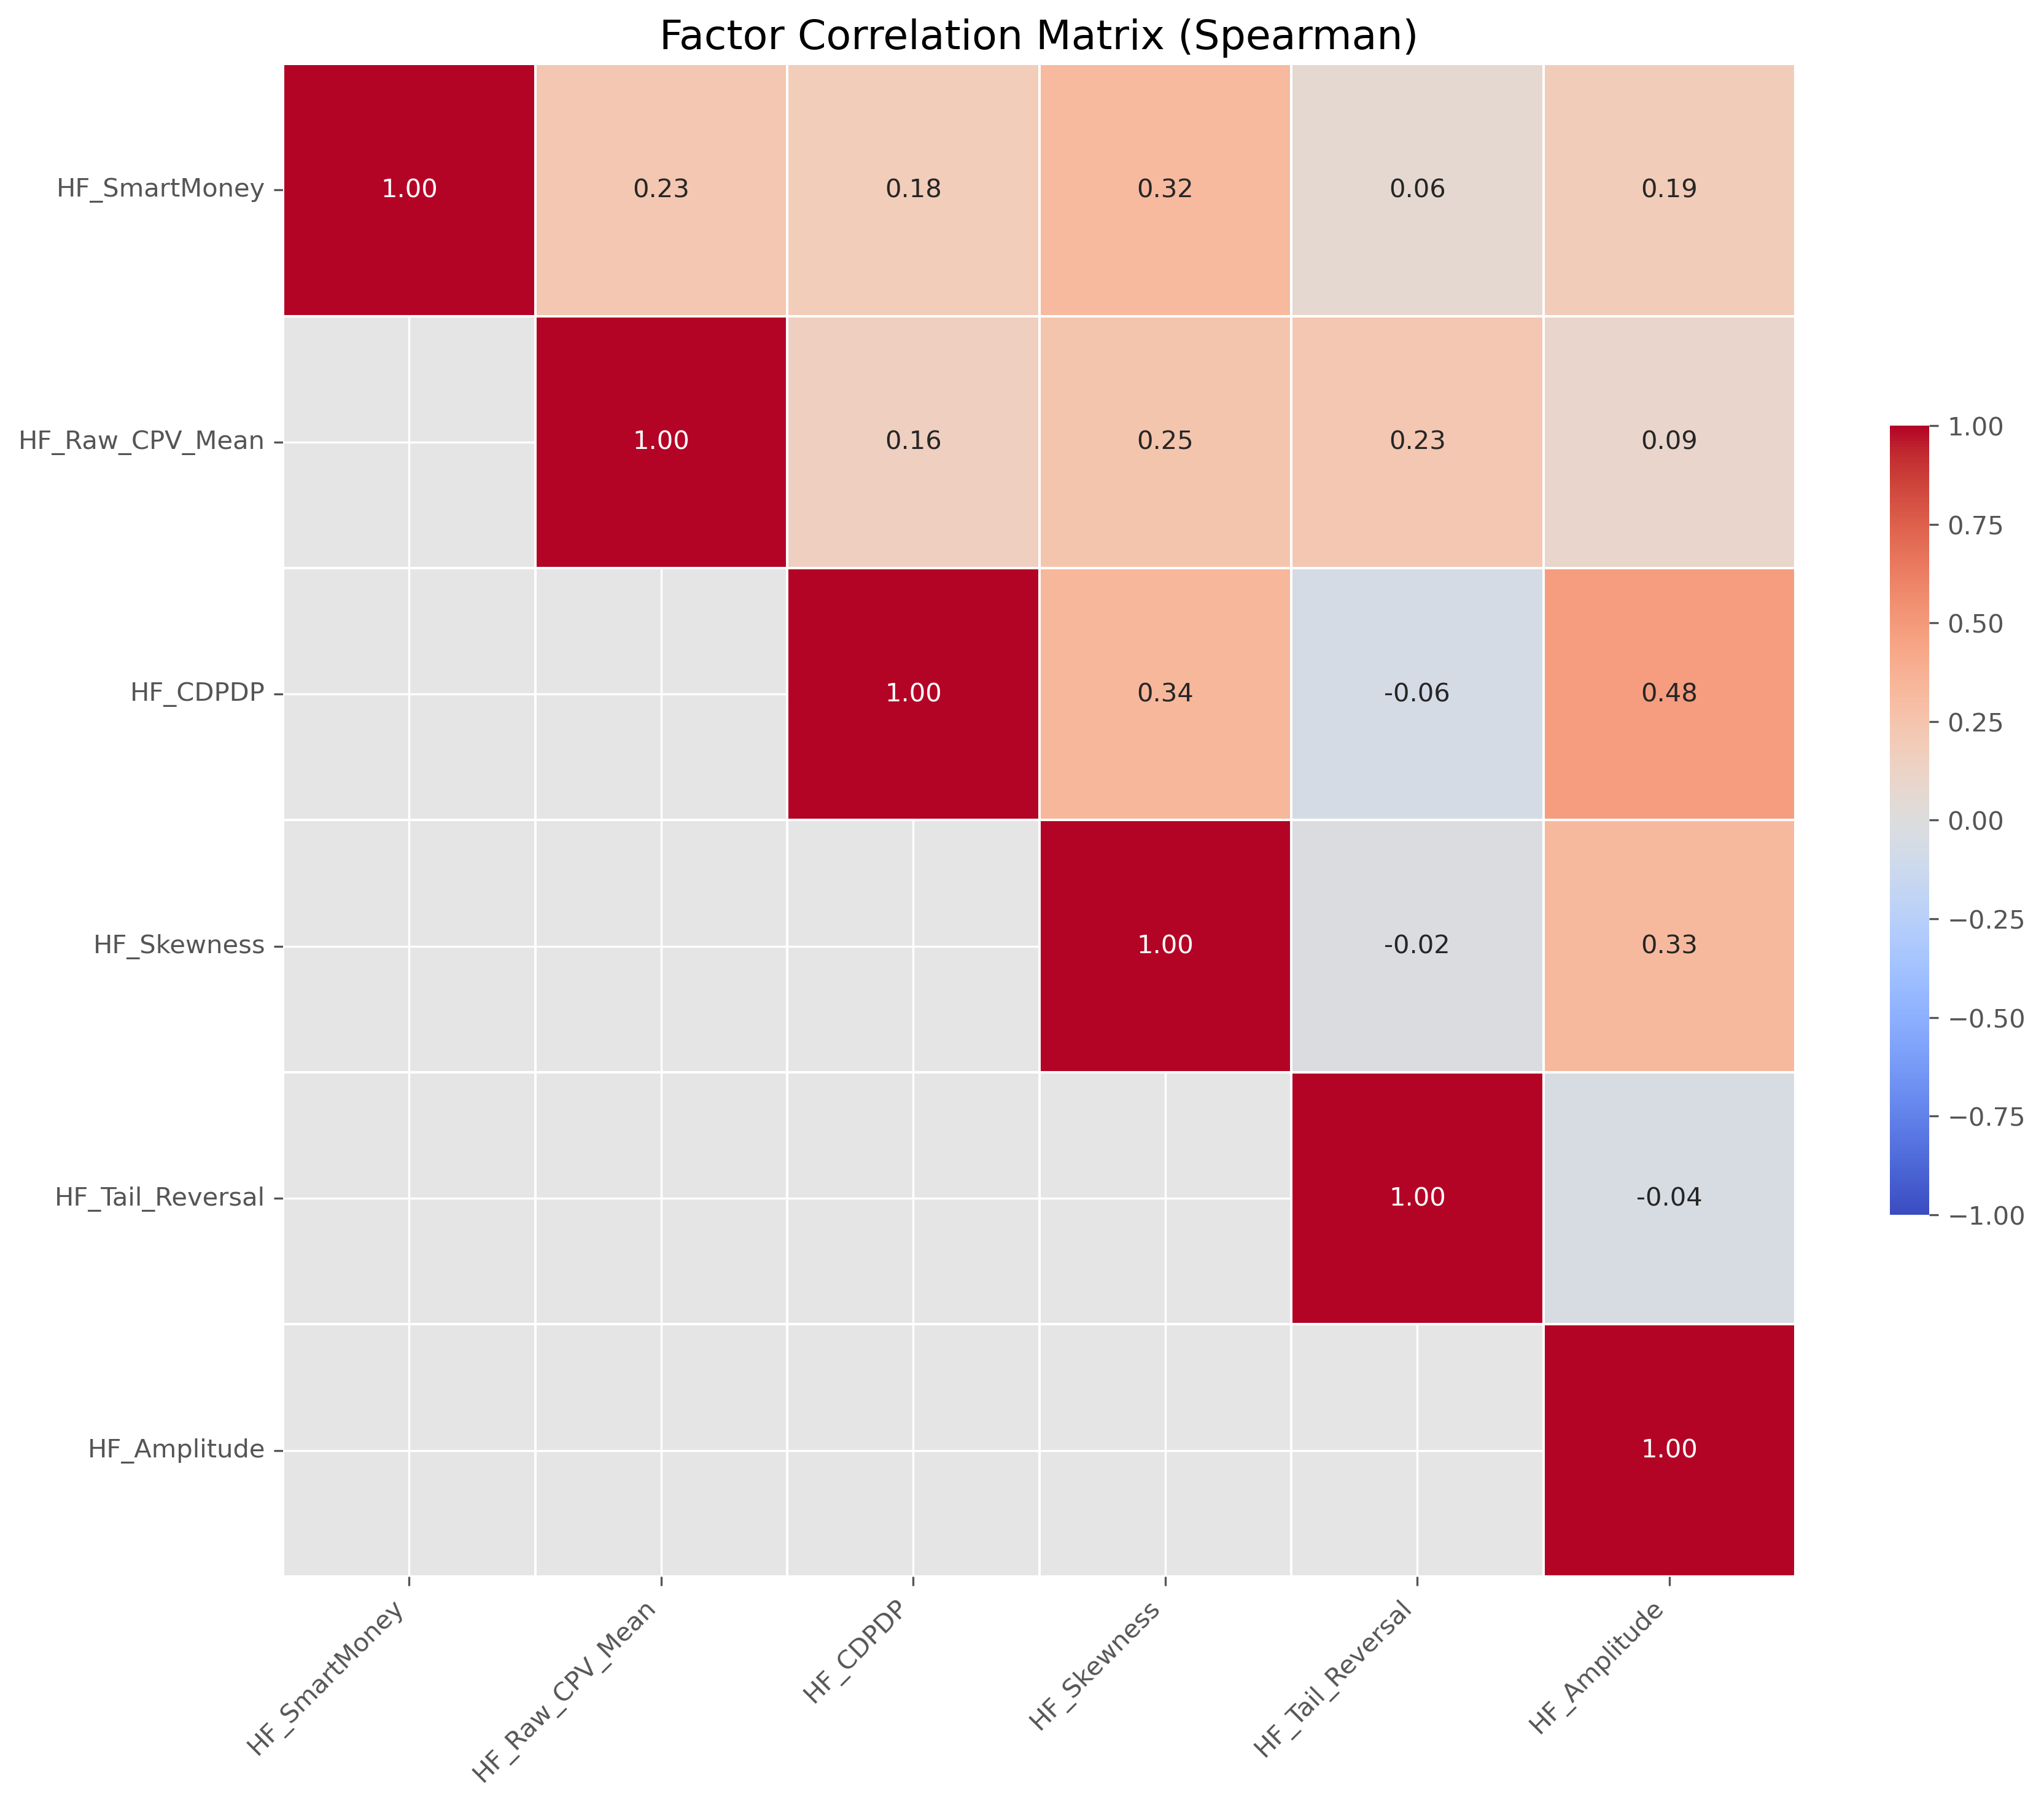
\includegraphics[width=0.82\linewidth]{Factor_Correlation_Matrix_spearman.png}
\end{figure}

\subsection{不同频度换仓下的因子测试}
\begin{table}[!h]
\centering
\caption{各因子在周频、双周频、月频下的绩效统计（手续费双边千三）}
\begin{tabular}{|l|c|cccccc|}
\hline
\rowcolor{headerblue} 
\textcolor{textwhite}{\textbf{频率}} & \textcolor{textwhite}{\textbf{因子指标}} & \textcolor{textwhite}{\textbf{IC}} & \textcolor{textwhite}{\textbf{RankIC}} & \textcolor{textwhite}{\textbf{年化收益}} & \textcolor{textwhite}{\textbf{收益波动比}} & \textcolor{textwhite}{\textbf{最大回撤}} & \textcolor{textwhite}{\textbf{月均换手}} \\ \hline

% --- Weekly 频率 ---
\rowcolor{rowgray}
& SmartMoney & -0.041 & -0.057 & 6.4\% & 1.18 & -4.0\% & 53.0\% \\ 
\rowcolor{rowgray}
& CPV\_Mean & -0.039 & -0.051 & 7.7\% & 1.30 & -3.9\% & 38.0\% \\ 
\rowcolor{rowgray}
& CDPDP & -0.029 & -0.044 & 4.1\% & 0.58 & -10.9\% & 26.0\% \\ 
\rowcolor{rowgray}
& Skewness & -0.037 & -0.053 & 6.8\% & 1.28 & -4.3\% & 35.0\% \\ 
\rowcolor{rowgray}
& Tail\_Reversal & -0.034 & -0.033 & 4.9\% & 0.81 & -8.1\% & 35.0\% \\ 
\rowcolor{rowgray}
& Amplitude & -0.021 & -0.045 & -2.9\% & -0.30 & -23.3\% & 18.0\% \\ 
\rowcolor{rowgray}
\multirow{-7}{*}{\textbf{Weekly}} & Pred\_Score & 0.046 & 0.050 & 10.8\% & 1.78 & -3.6\% & 47.0\% \\ \hline

% --- BiWeekly 频率 ---
& SmartMoney & -0.038 & -0.058 & 5.8\% & 0.97 & -7.4\% & 76.0\% \\ 
& CPV\_Mean & -0.044 & -0.056 & 11.4\% & 1.91 & -3.3\% & 54.0\% \\ 
& CDPDP & -0.039 & -0.057 & 12.3\% & 1.70 & -7.4\% & 38.0\% \\ 
& Skewness & -0.045 & -0.059 & 11.8\% & 2.25 & -2.6\% & 50.0\% \\ 
& Tail\_Reversal & -0.035 & -0.030 & 5.3\% & 0.89 & -8.6\% & 50.0\% \\ 
& Amplitude & -0.030 & -0.054 & 4.0\% & 0.42 & -13.9\% & 29.0\% \\ 
\multirow{-7}{*}{\textbf{BiWeekly}} & Pred\_Score & 0.045 & 0.045 & \textbf{14.8\%} & \textbf{2.61} & \textbf{-2.0\%} & 58.0\% \\ \hline

% --- Monthly 频率 ---
\rowcolor{rowgray}
& SmartMoney & -0.037 & -0.052 & 6.2\% & 1.11 & -7.5\% & 77.0\% \\ 
\rowcolor{rowgray}
& CPV\_Mean & -0.047 & -0.059 & 11.8\% & 2.14 & -3.7\% & 75.0\% \\ 
\rowcolor{rowgray}
& CDPDP & -0.044 & -0.064 & 12.2\% & 1.99 & -3.8\% & 55.0\% \\ 
\rowcolor{rowgray}
& Skewness & -0.054 & \textbf{-0.070} & \textbf{12.6\%} & 2.60 & -3.7\% & 72.0\% \\ 
\rowcolor{rowgray}
& Tail\_Reversal & -0.033 & -0.028 & 5.1\% & 0.89 & -7.2\% & 71.0\% \\ 
\rowcolor{rowgray}
& Amplitude & -0.038 & -0.066 & 7.2\% & 0.86 & -10.2\% & 44.0\% \\ 
\rowcolor{rowgray}
\multirow{-7}{*}{\textbf{Monthly}} & Pred\_Score & 0.029 & 0.045 & 8.5\% & 1.65 & -4.4\% & 71.0\% \\ \hline
\end{tabular}
\end{table}
\newpage
本部分展示了各因子在不同持有期（周频、双周频、月频）下的表现。
\begin{itemize}
    \item \textbf{HF\_Skewness（偏度）}：表现最为优异，月频RankIC达到-0.070，年化收益12.6\%。这有力地验证了A股市场存在显著的博彩效应，高偏度股票后续表现疲软。
    \item \textbf{HF\_Raw\_CPV\_Mean}：在双周频和月频均表现稳定（收益率 >11\%），说明日内“量价背离”或“量价齐升”的过度反应是稳定的反向指标。
    \item \textbf{HF\_Amplitude（振幅）}：该因子表现出明显的期限结构差异。在周频下收益为负（-2.9\%），但在月频下转正（7.2\%）。这可能意味着短期内高振幅代表情绪宣泄后的动量衰竭，而拉长周期看，高波动率可能包含风险溢价，或需配合其他指标使用。
    \item \textbf{多因子组合效果 (XGBoost)}：利用XGBoost模型对上述高频因子进行非线性合成，生成的\texttt{Pred\_Score}在双周频（BiWeekly）策略下取得了最佳平衡。相比单因子，组合模型显著降低了回撤，表明各高频因子之间存在较低的相关性，能够通过非线性组合互补。
\end{itemize}

\begin{figure}[!h]
    \centering
    % 第一行：SmartMoney 与 CPV
    \begin{minipage}[b]{0.48\linewidth}
        \centering
        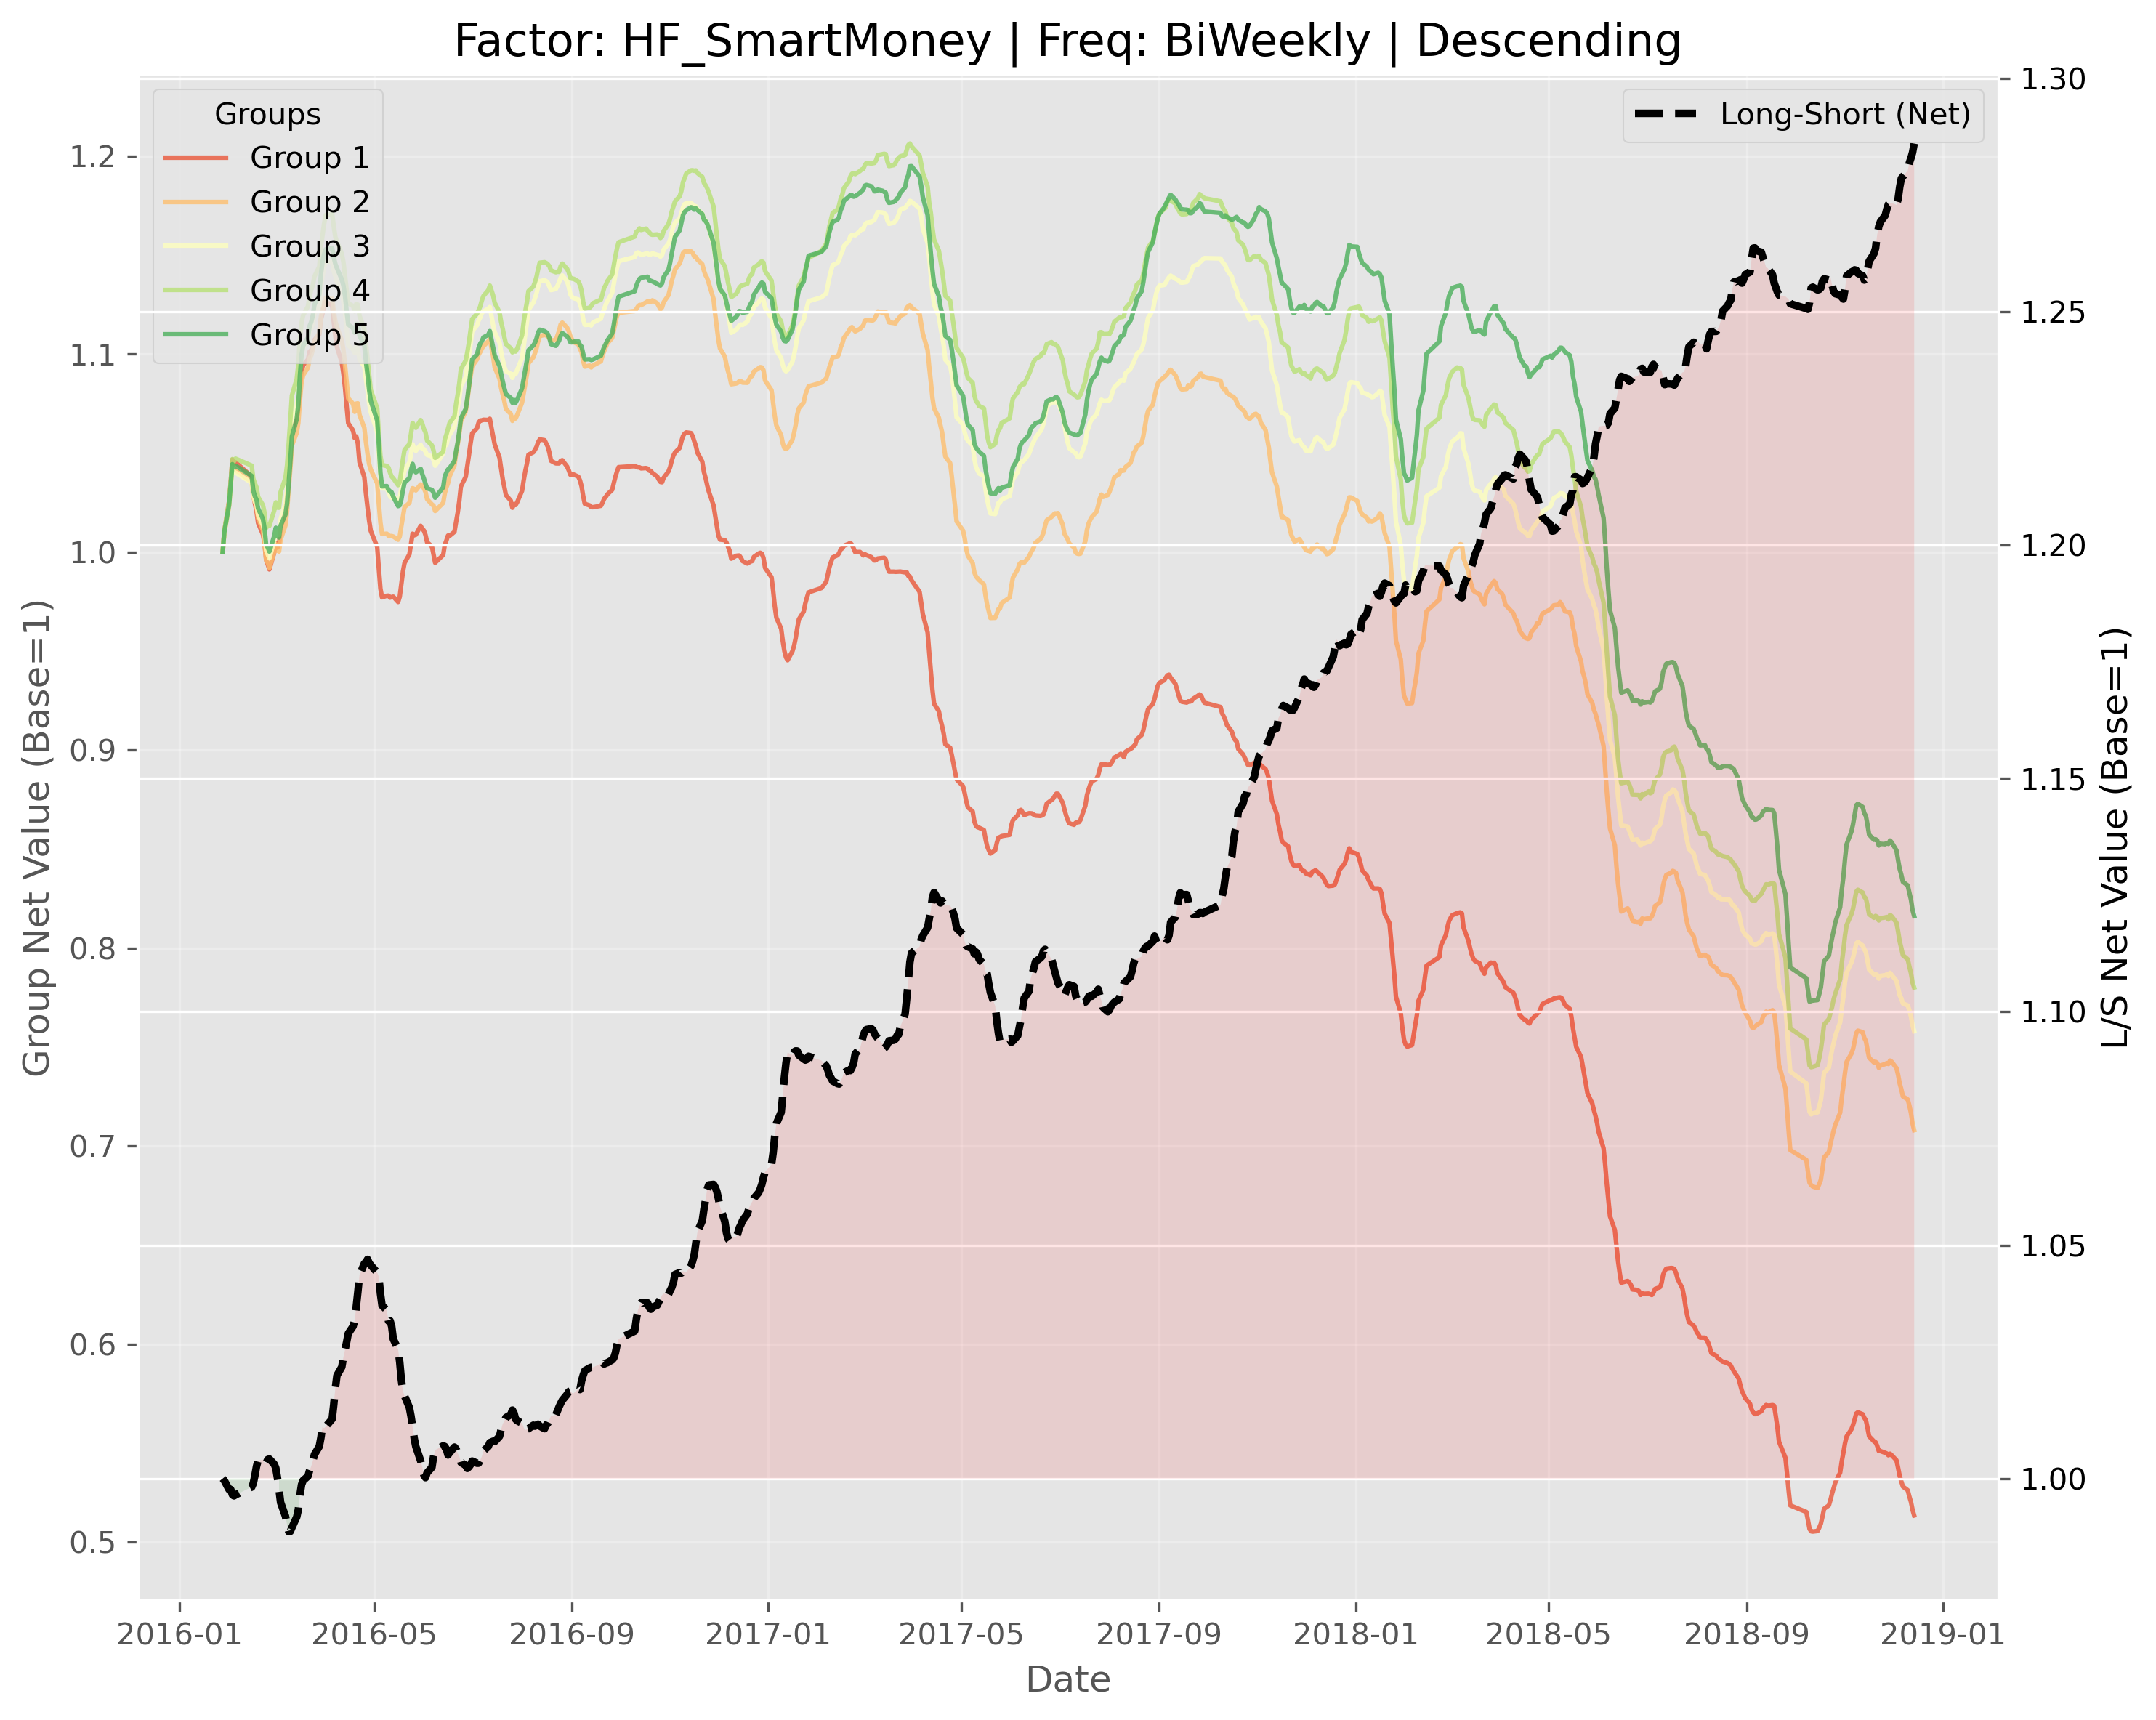
\includegraphics[width=\textwidth]{Factor_HF_SmartMoney_-_Freq_BiWeekly_-_Descending.png}
    \end{minipage}
    \hfill
    \begin{minipage}[b]{0.48\linewidth}
        \centering
        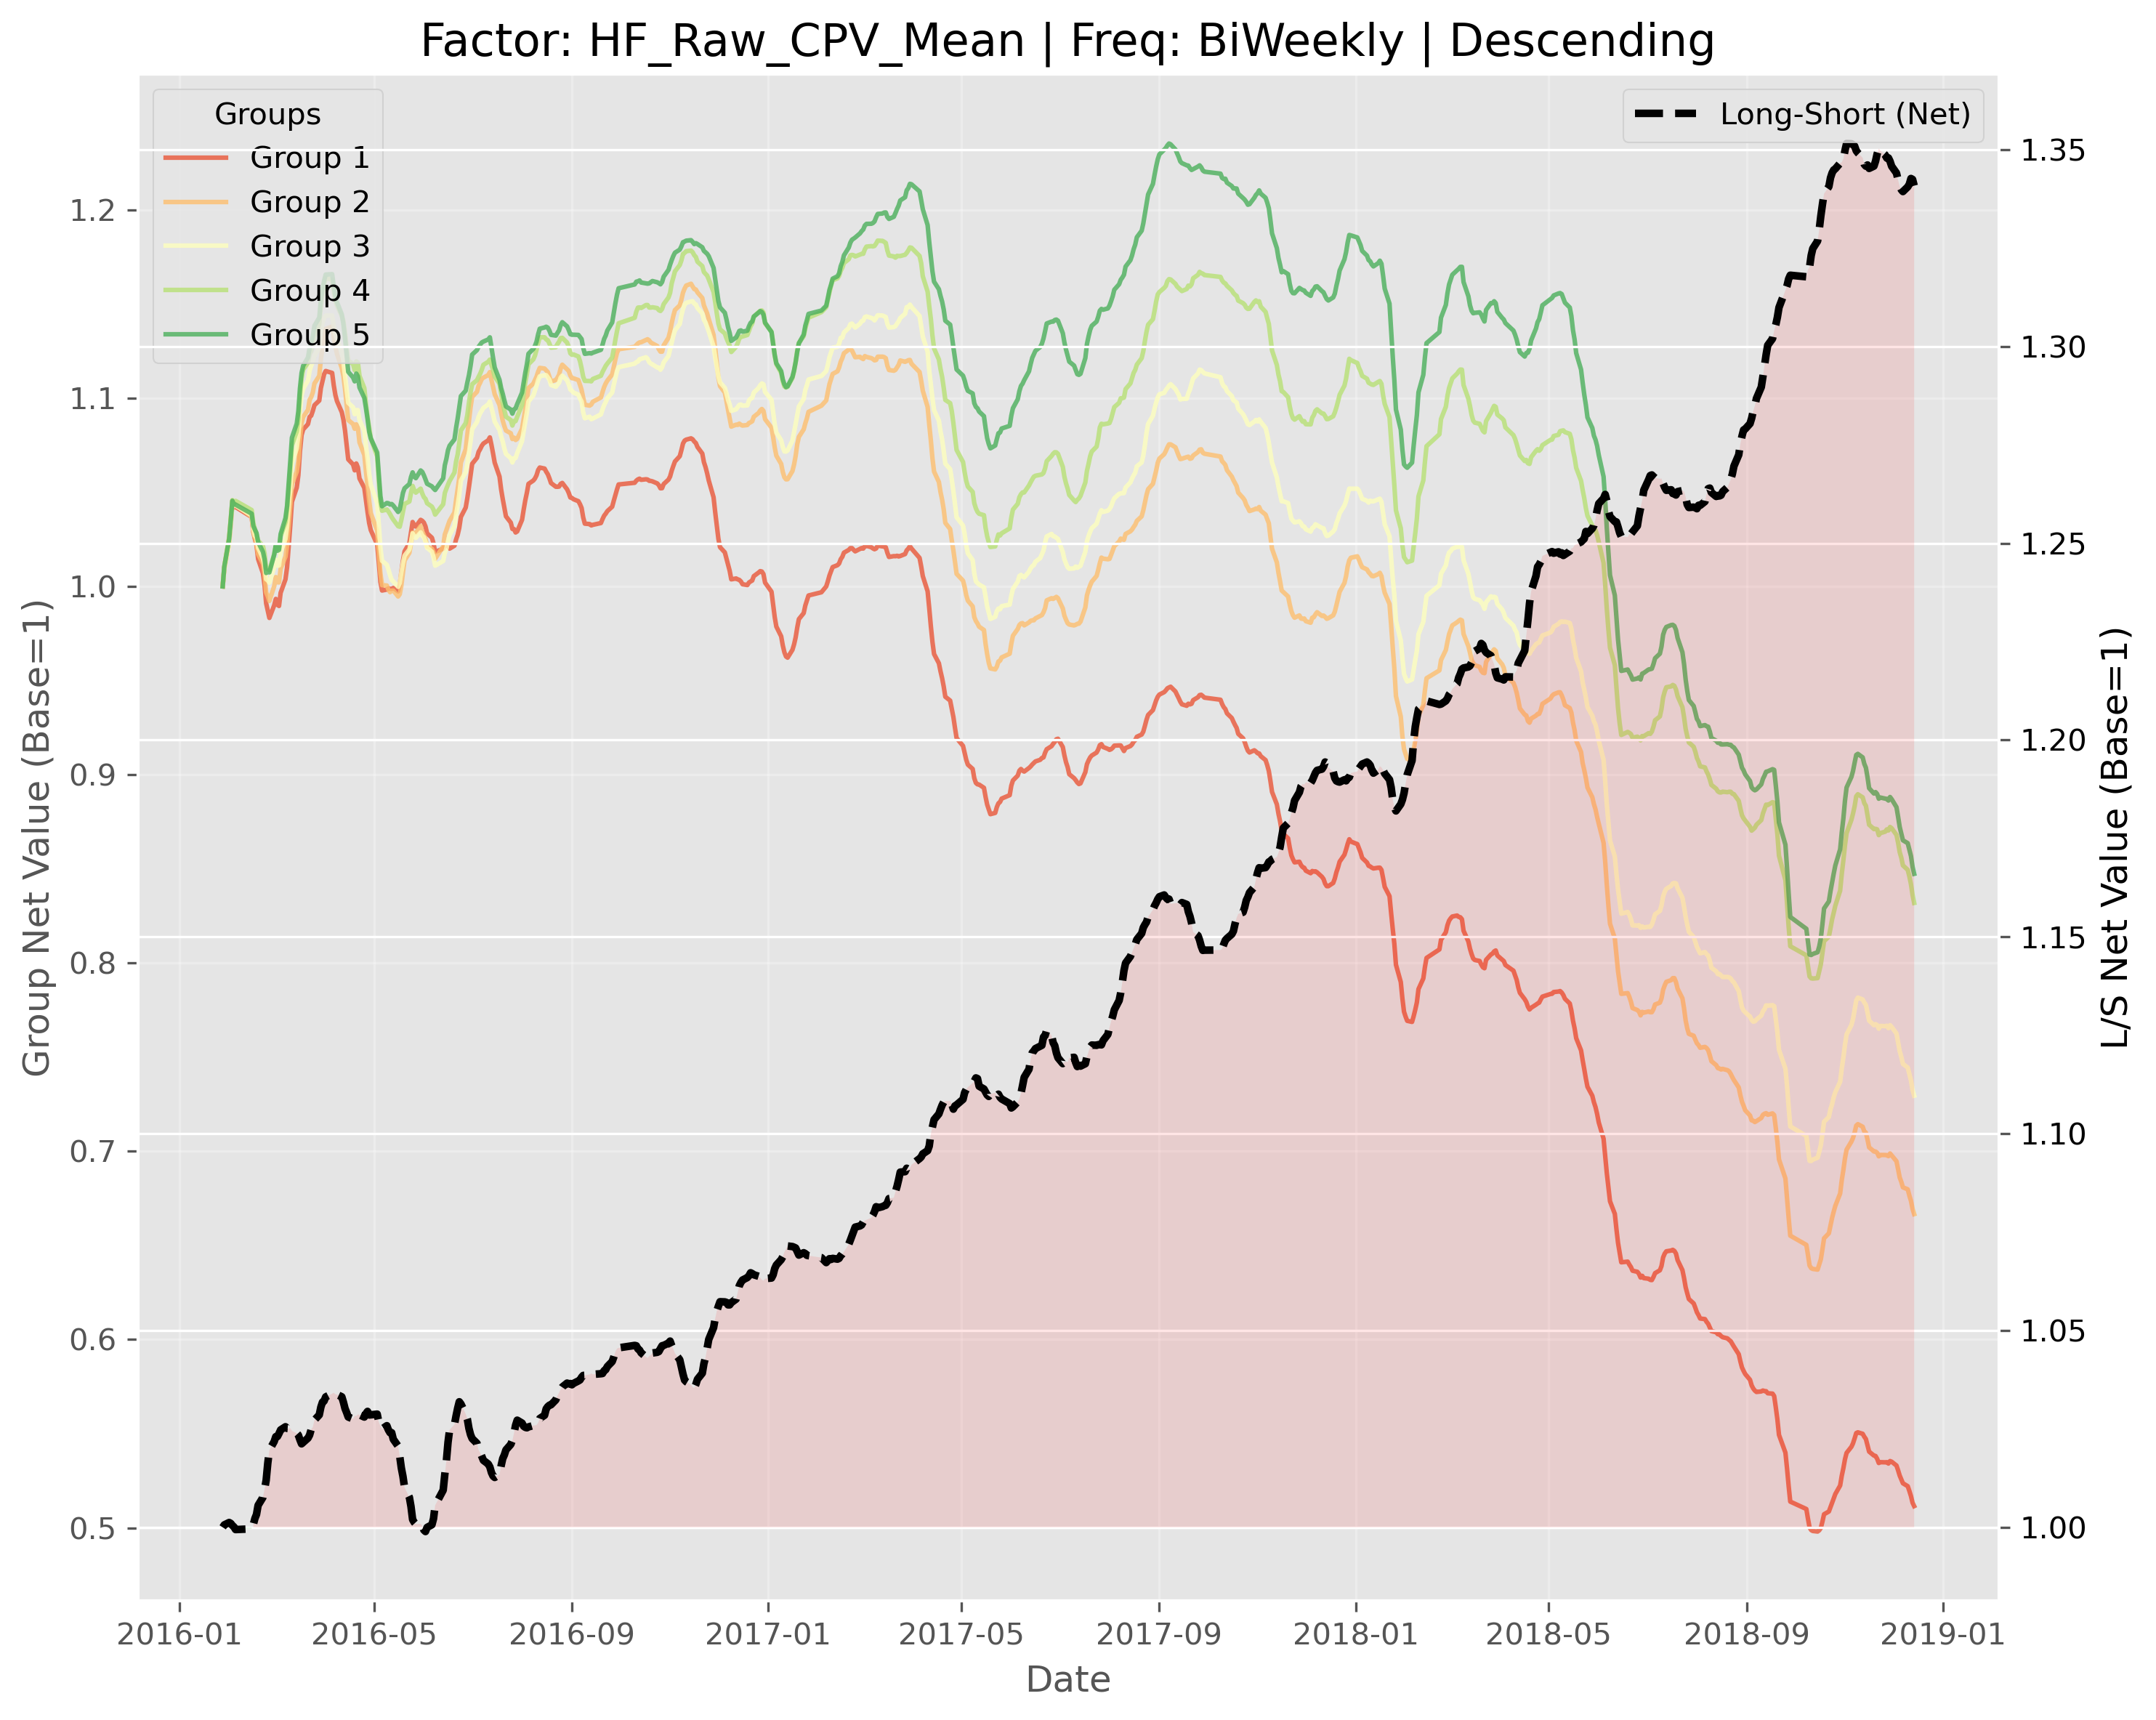
\includegraphics[width=\textwidth]{Factor_HF_Raw_CPV_Mean_-_Freq_BiWeekly_-_Descending.png}
    \end{minipage}
\end{figure}
    \vspace{1.5em} % 设置行间距
\begin{figure}[!h]
    % 第二行：CDPDP 与 Skewness
    \begin{minipage}[b]{0.48\linewidth}
        \centering
        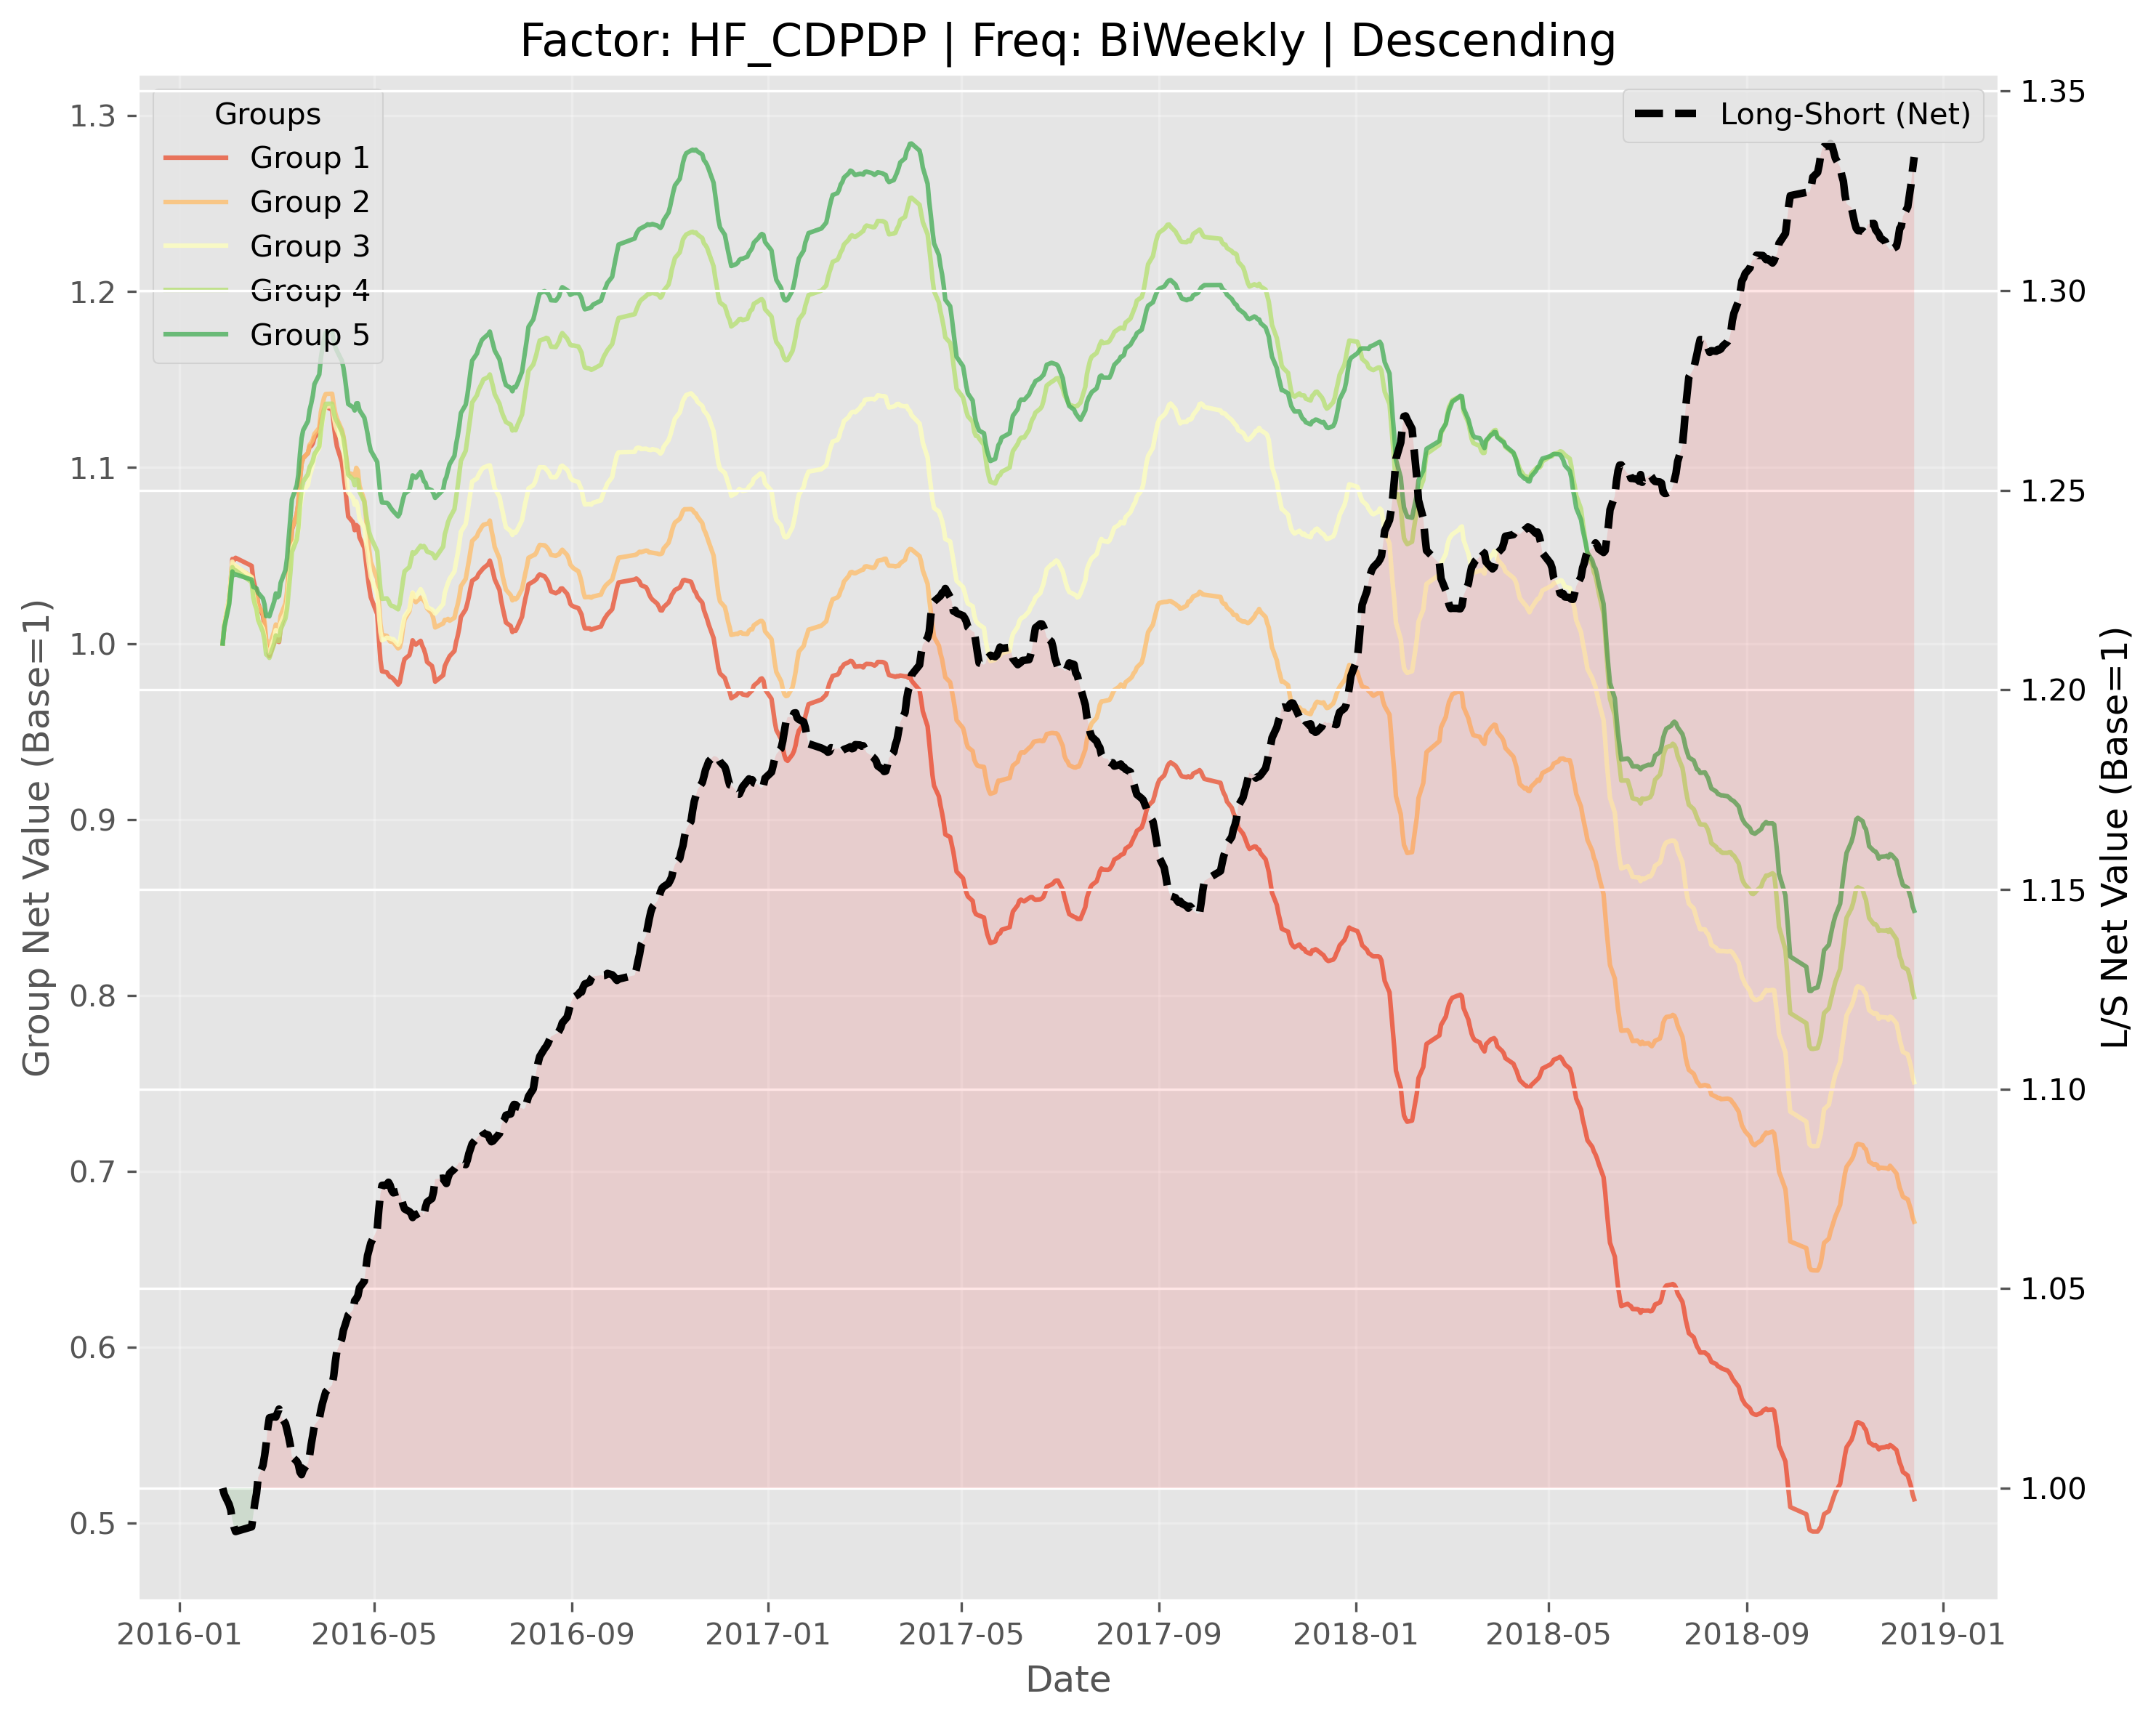
\includegraphics[width=\textwidth]{Factor_HF_CDPDP_-_Freq_BiWeekly_-_Descending.png}
    \end{minipage}
    \hfill
    \begin{minipage}[b]{0.48\linewidth}
        \centering
        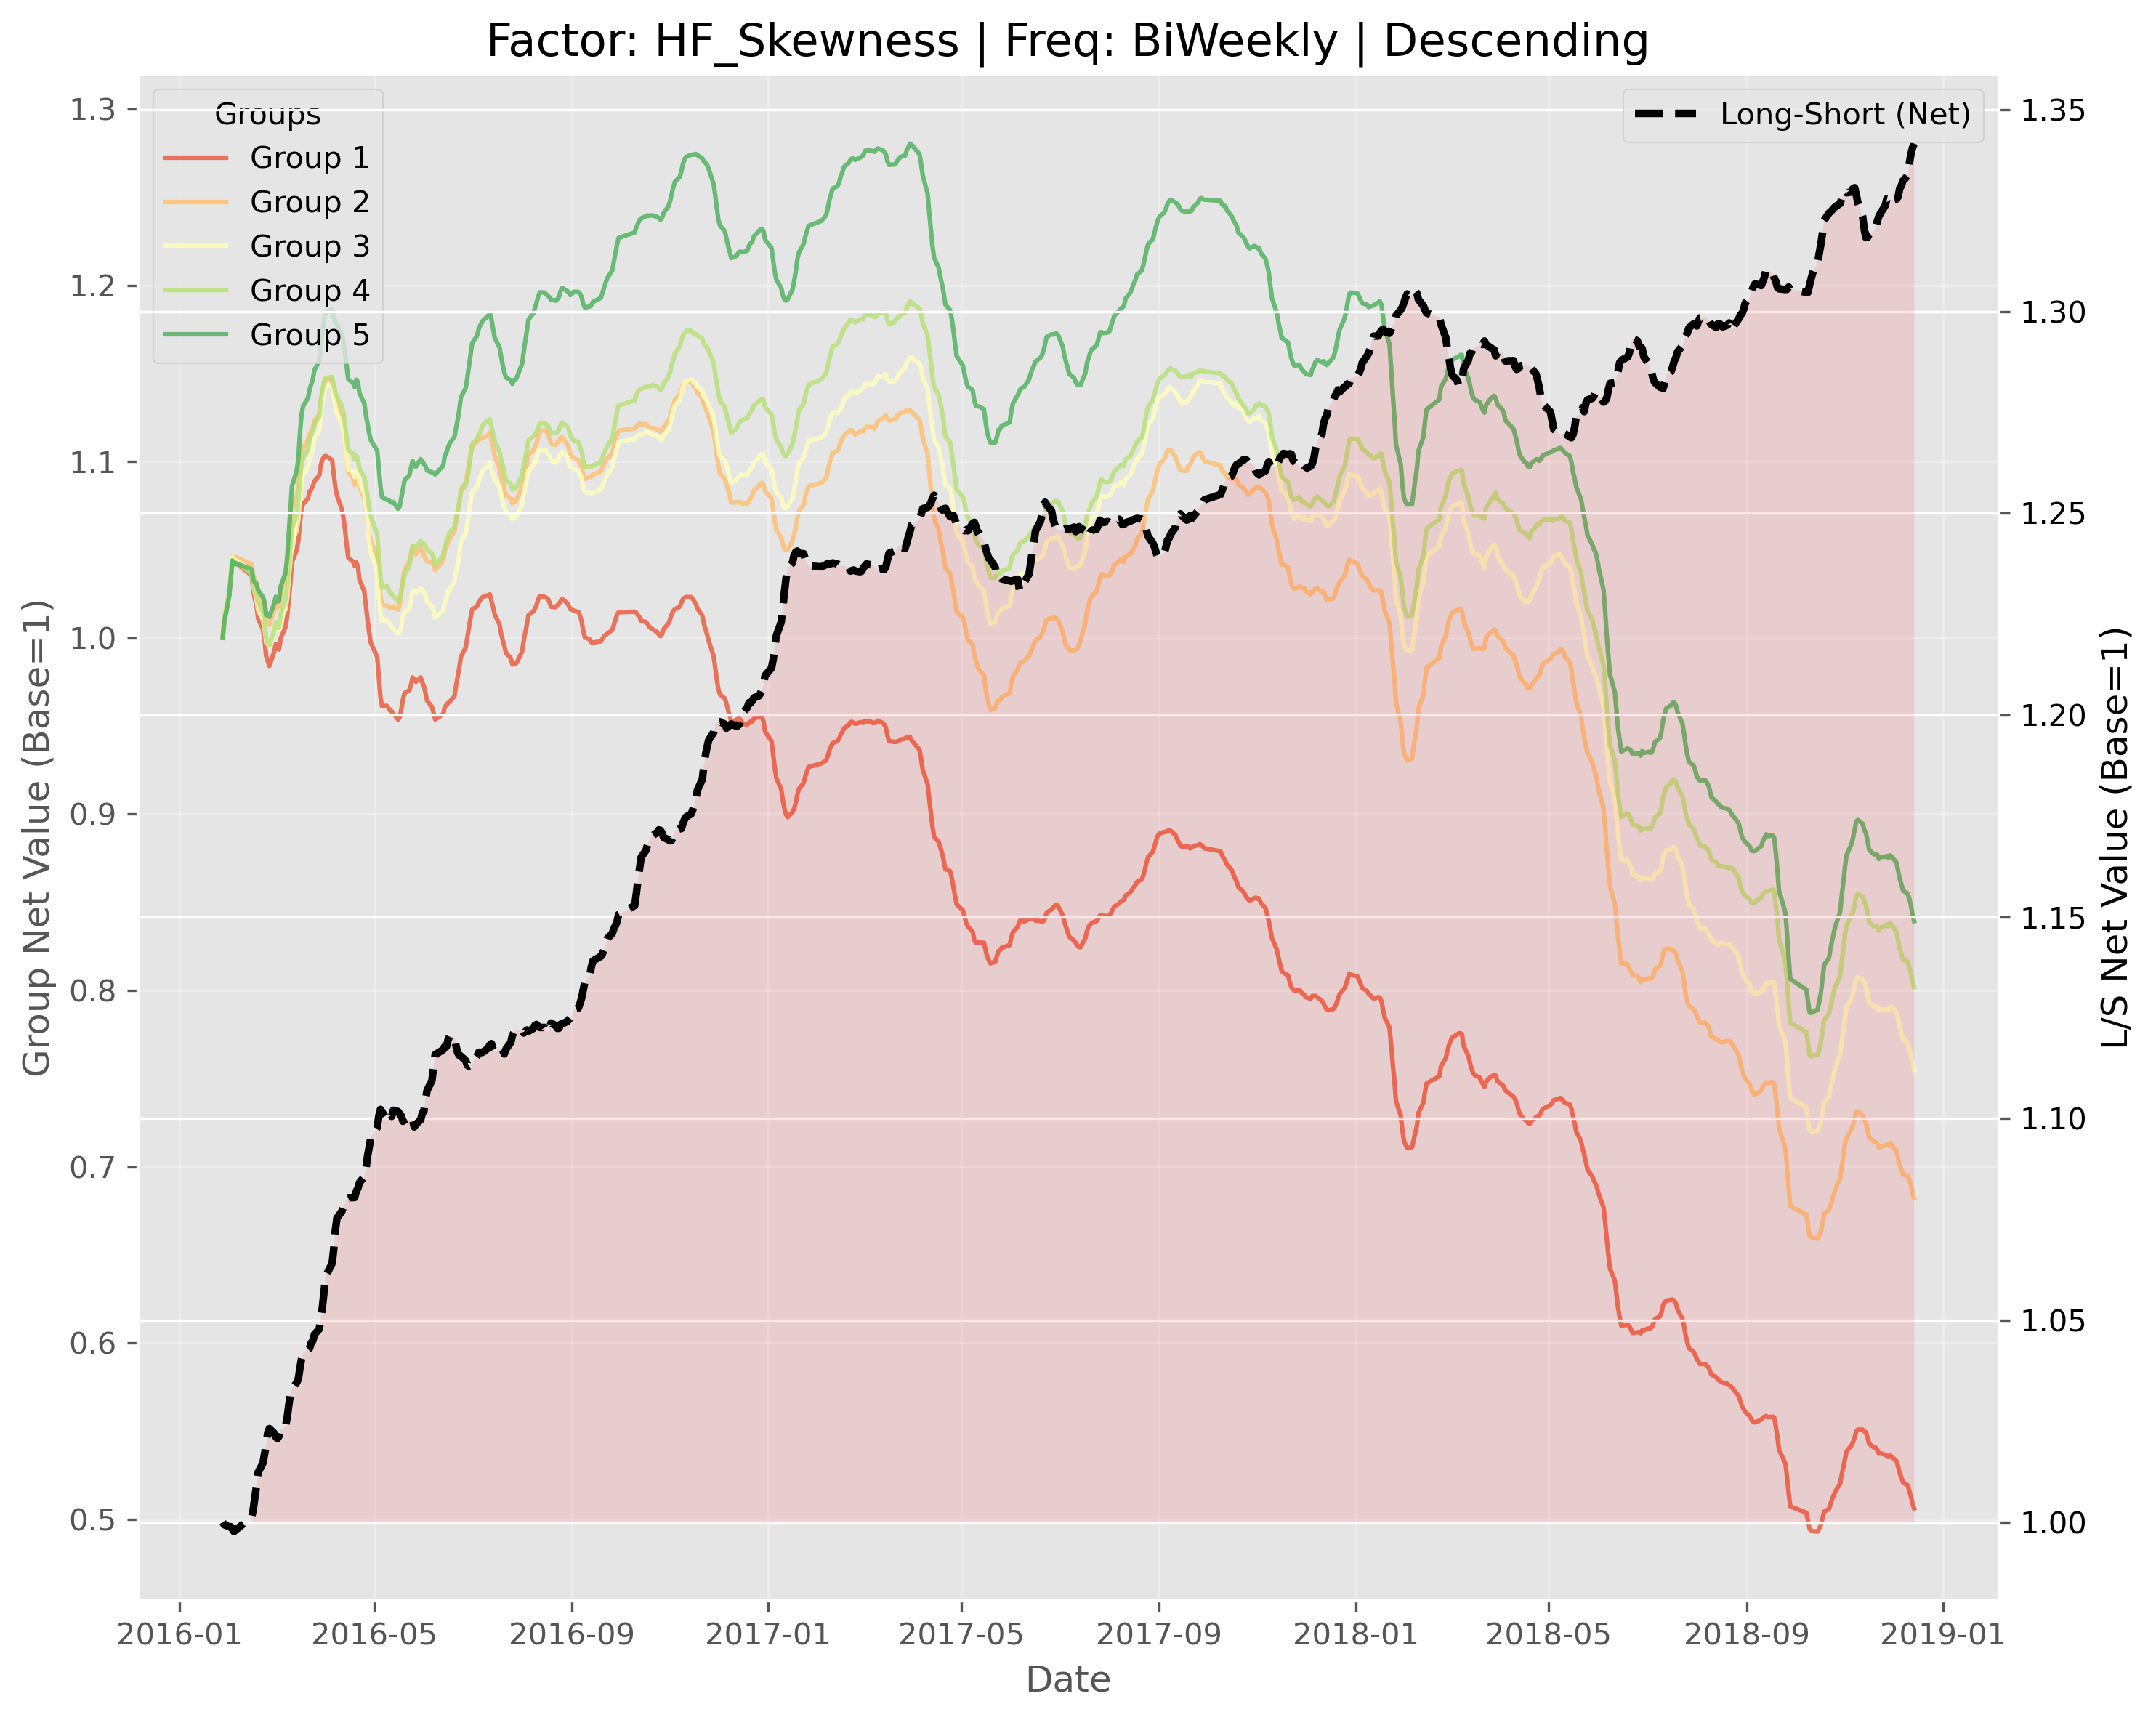
\includegraphics[width=\textwidth]{Factor_HF_Skewness_-_Freq_BiWeekly_-_Descending.png}
    \end{minipage}
\end{figure}
    \vspace{1.5em}
\begin{figure}[!h]
    % 第三行：Tail Reversal 与 Amplitude
    \begin{minipage}[b]{0.48\linewidth}
        \centering
        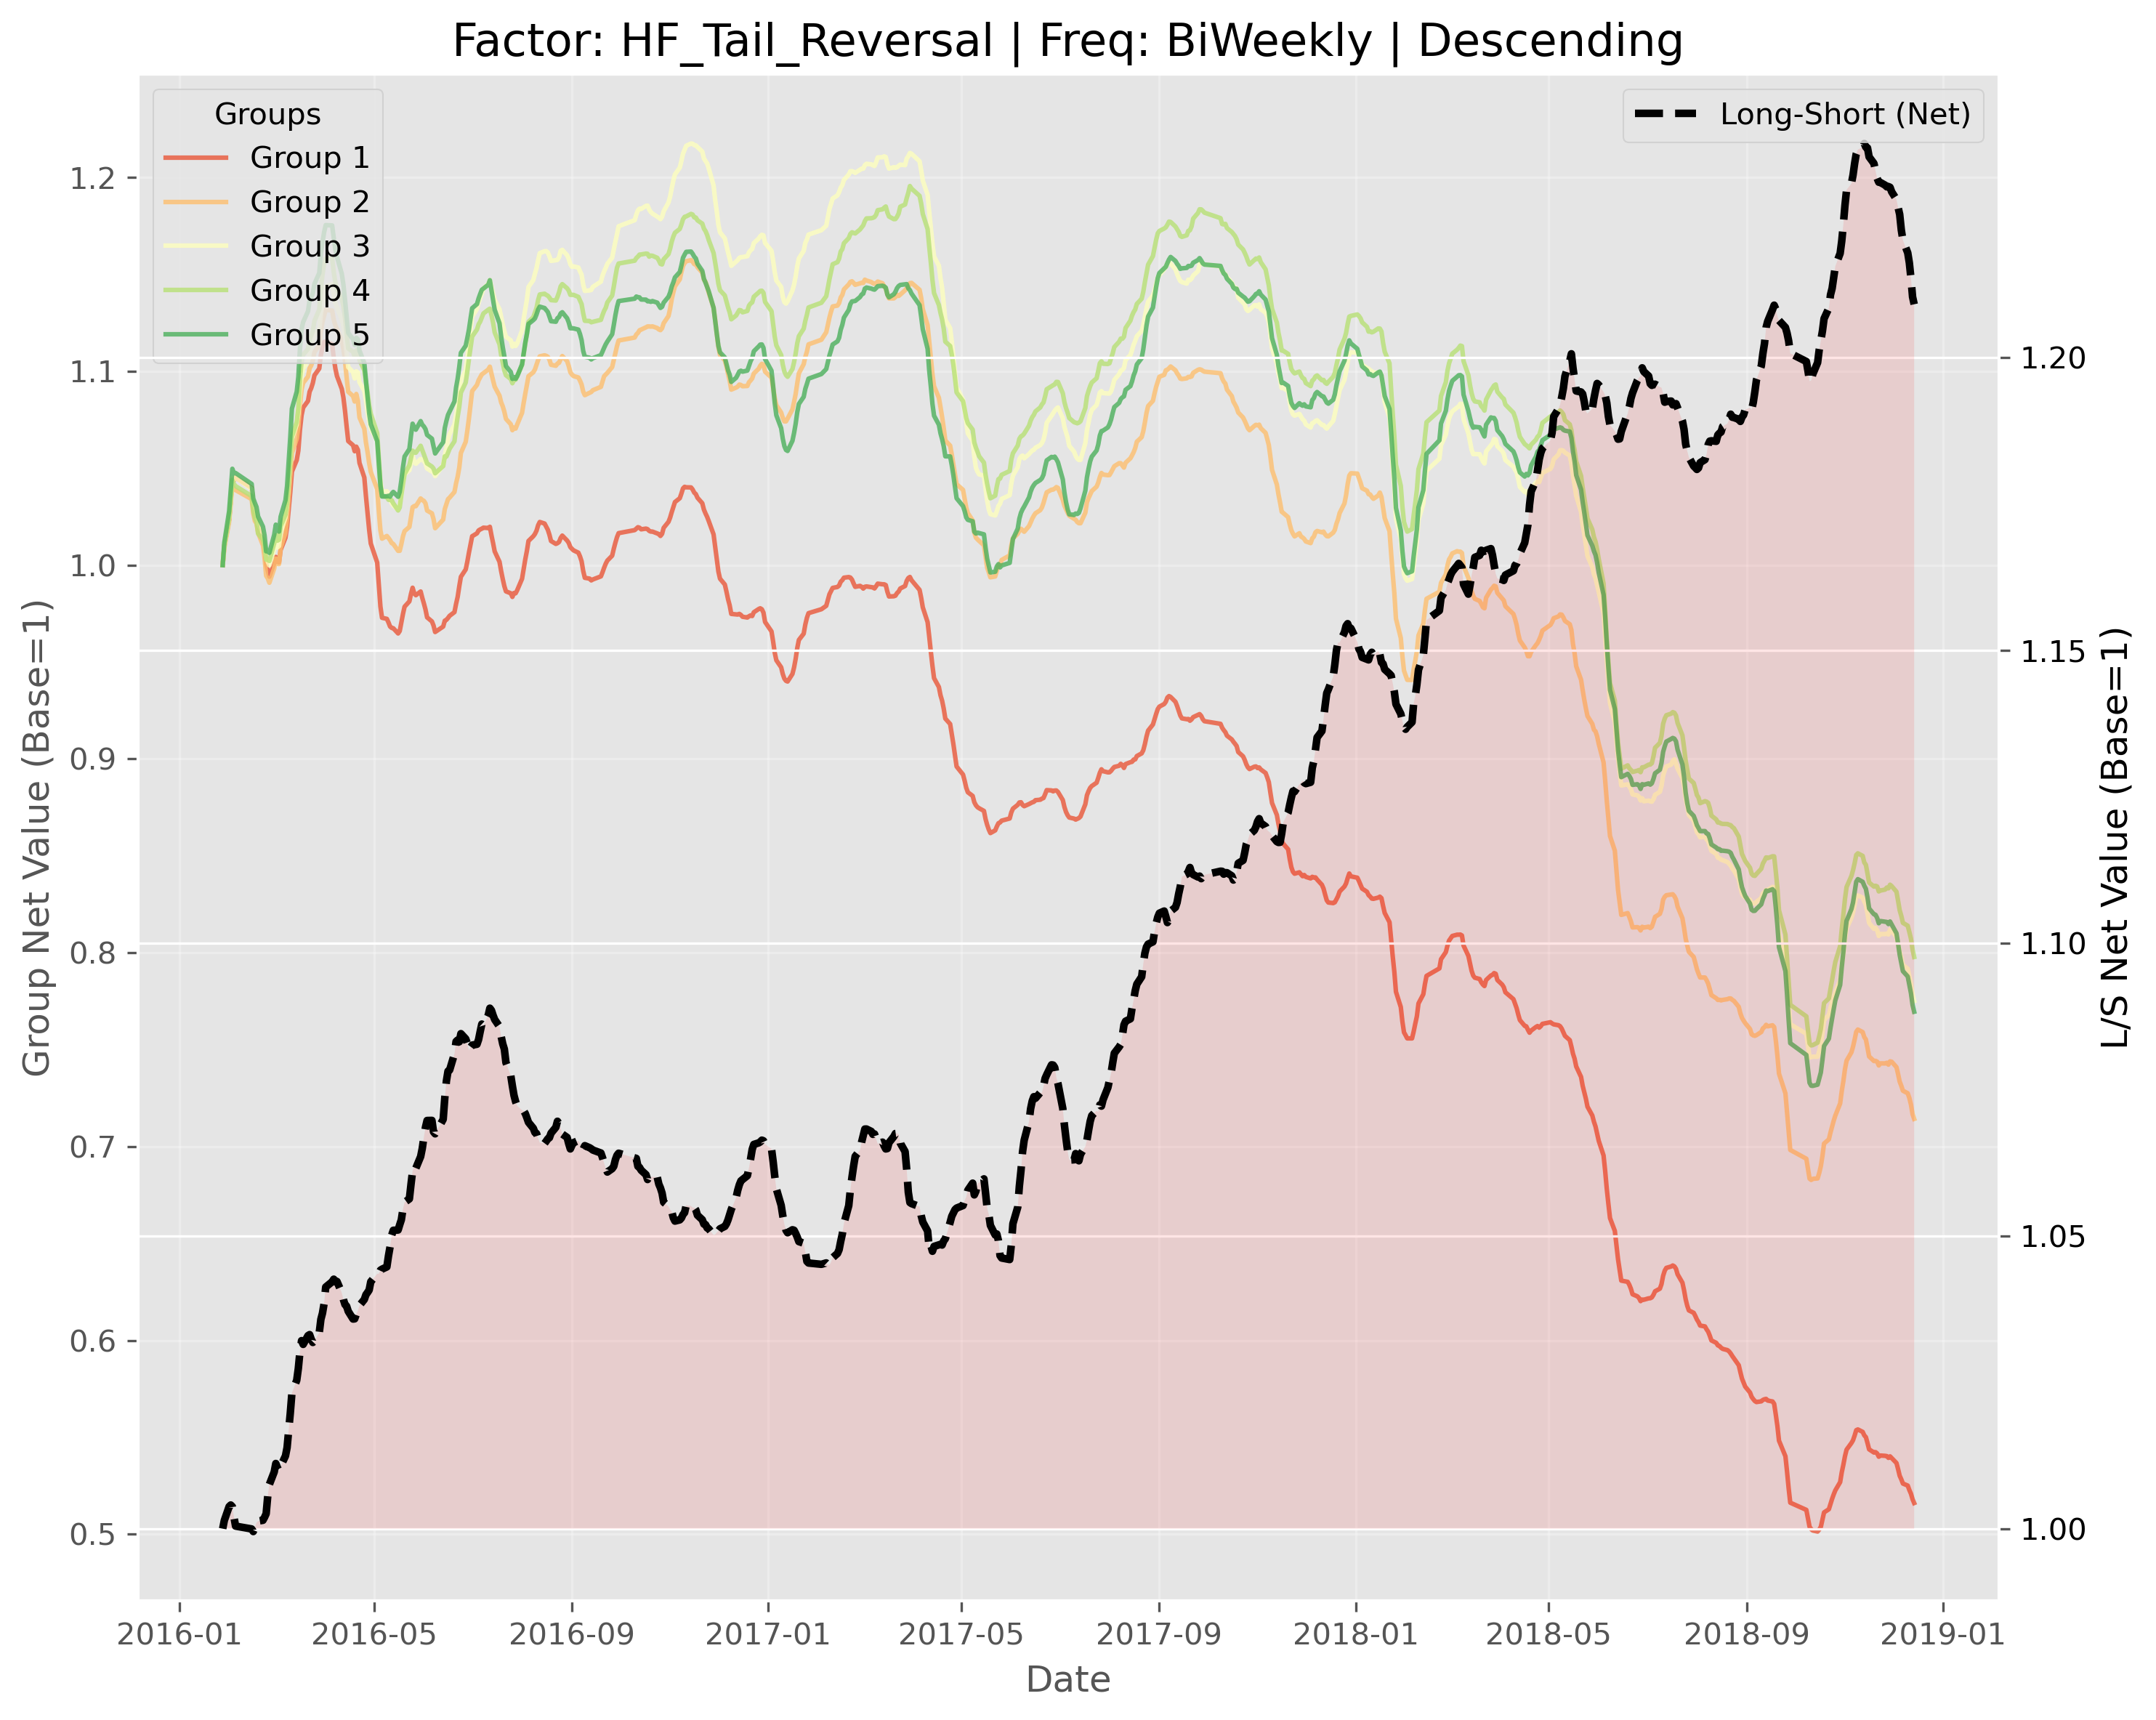
\includegraphics[width=\textwidth]{Factor_HF_Tail_Reversal_-_Freq_BiWeekly_-_Descending.png}
    \end{minipage}
    \hfill
    \begin{minipage}[b]{0.48\linewidth}
        \centering
        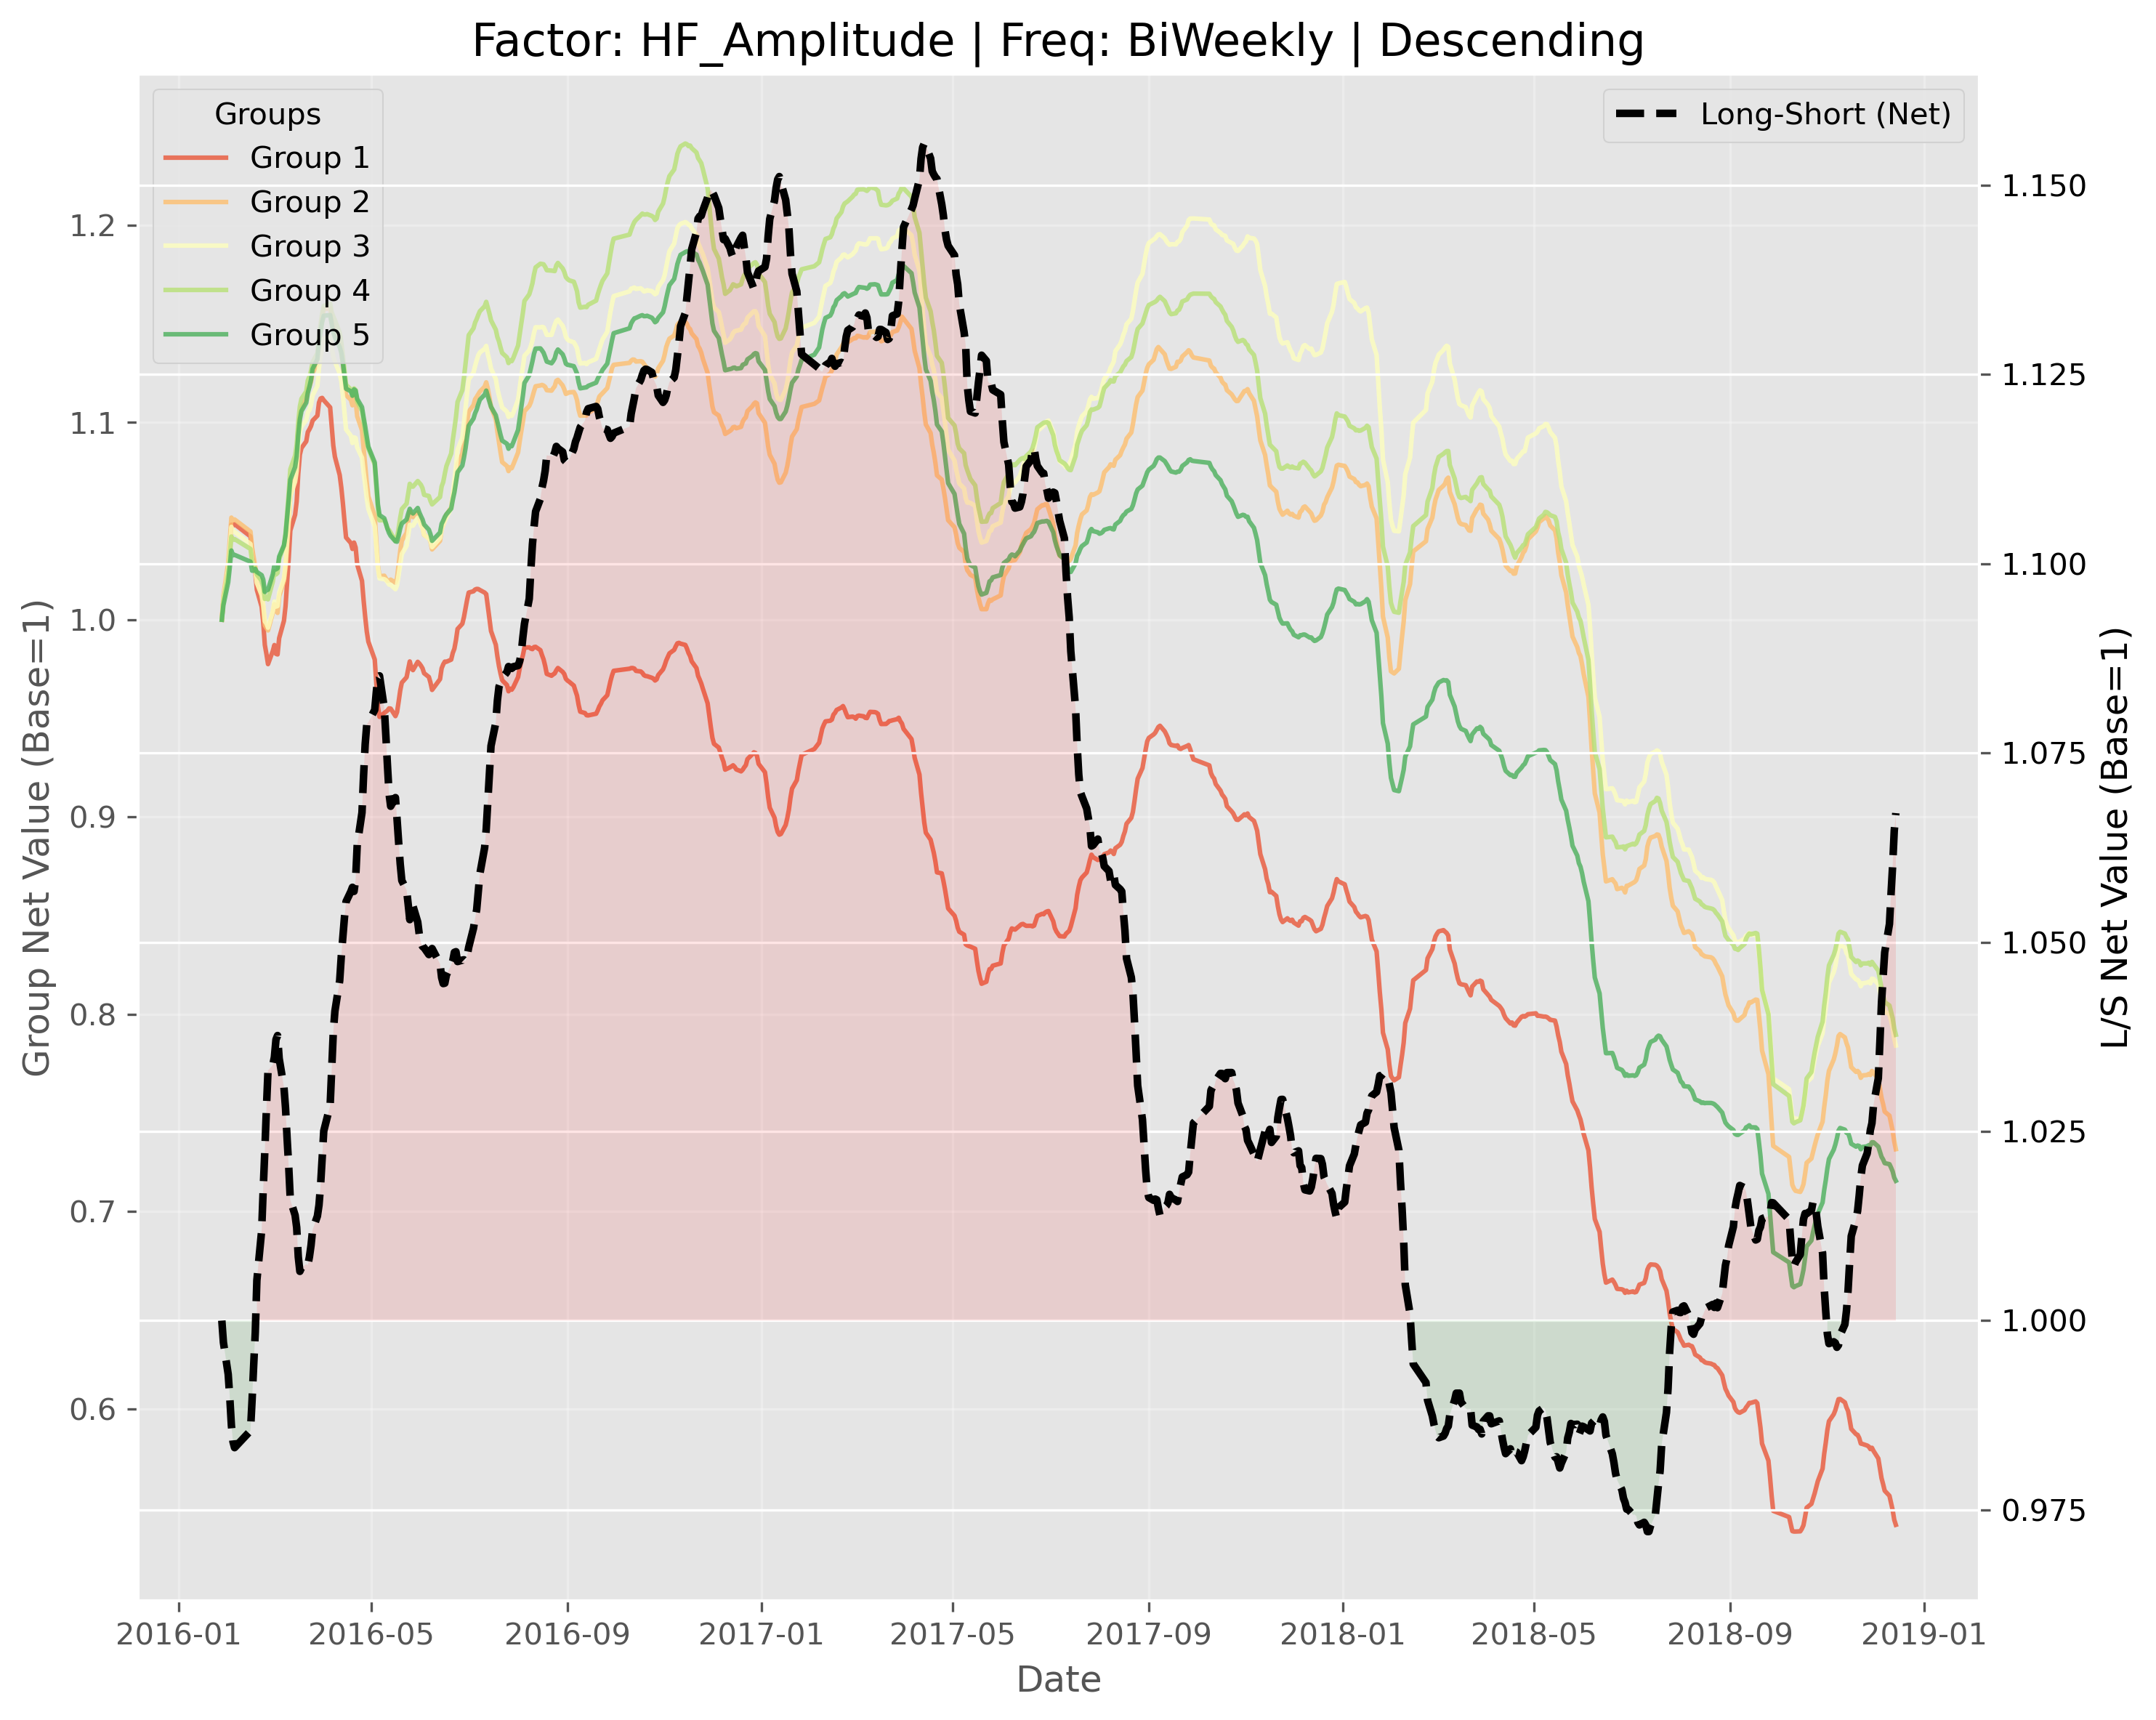
\includegraphics[width=\textwidth]{Factor_HF_Amplitude_-_Freq_BiWeekly_-_Descending.png}
    \end{minipage}
\end{figure}

\begin{figure}[!h]
    \centering
    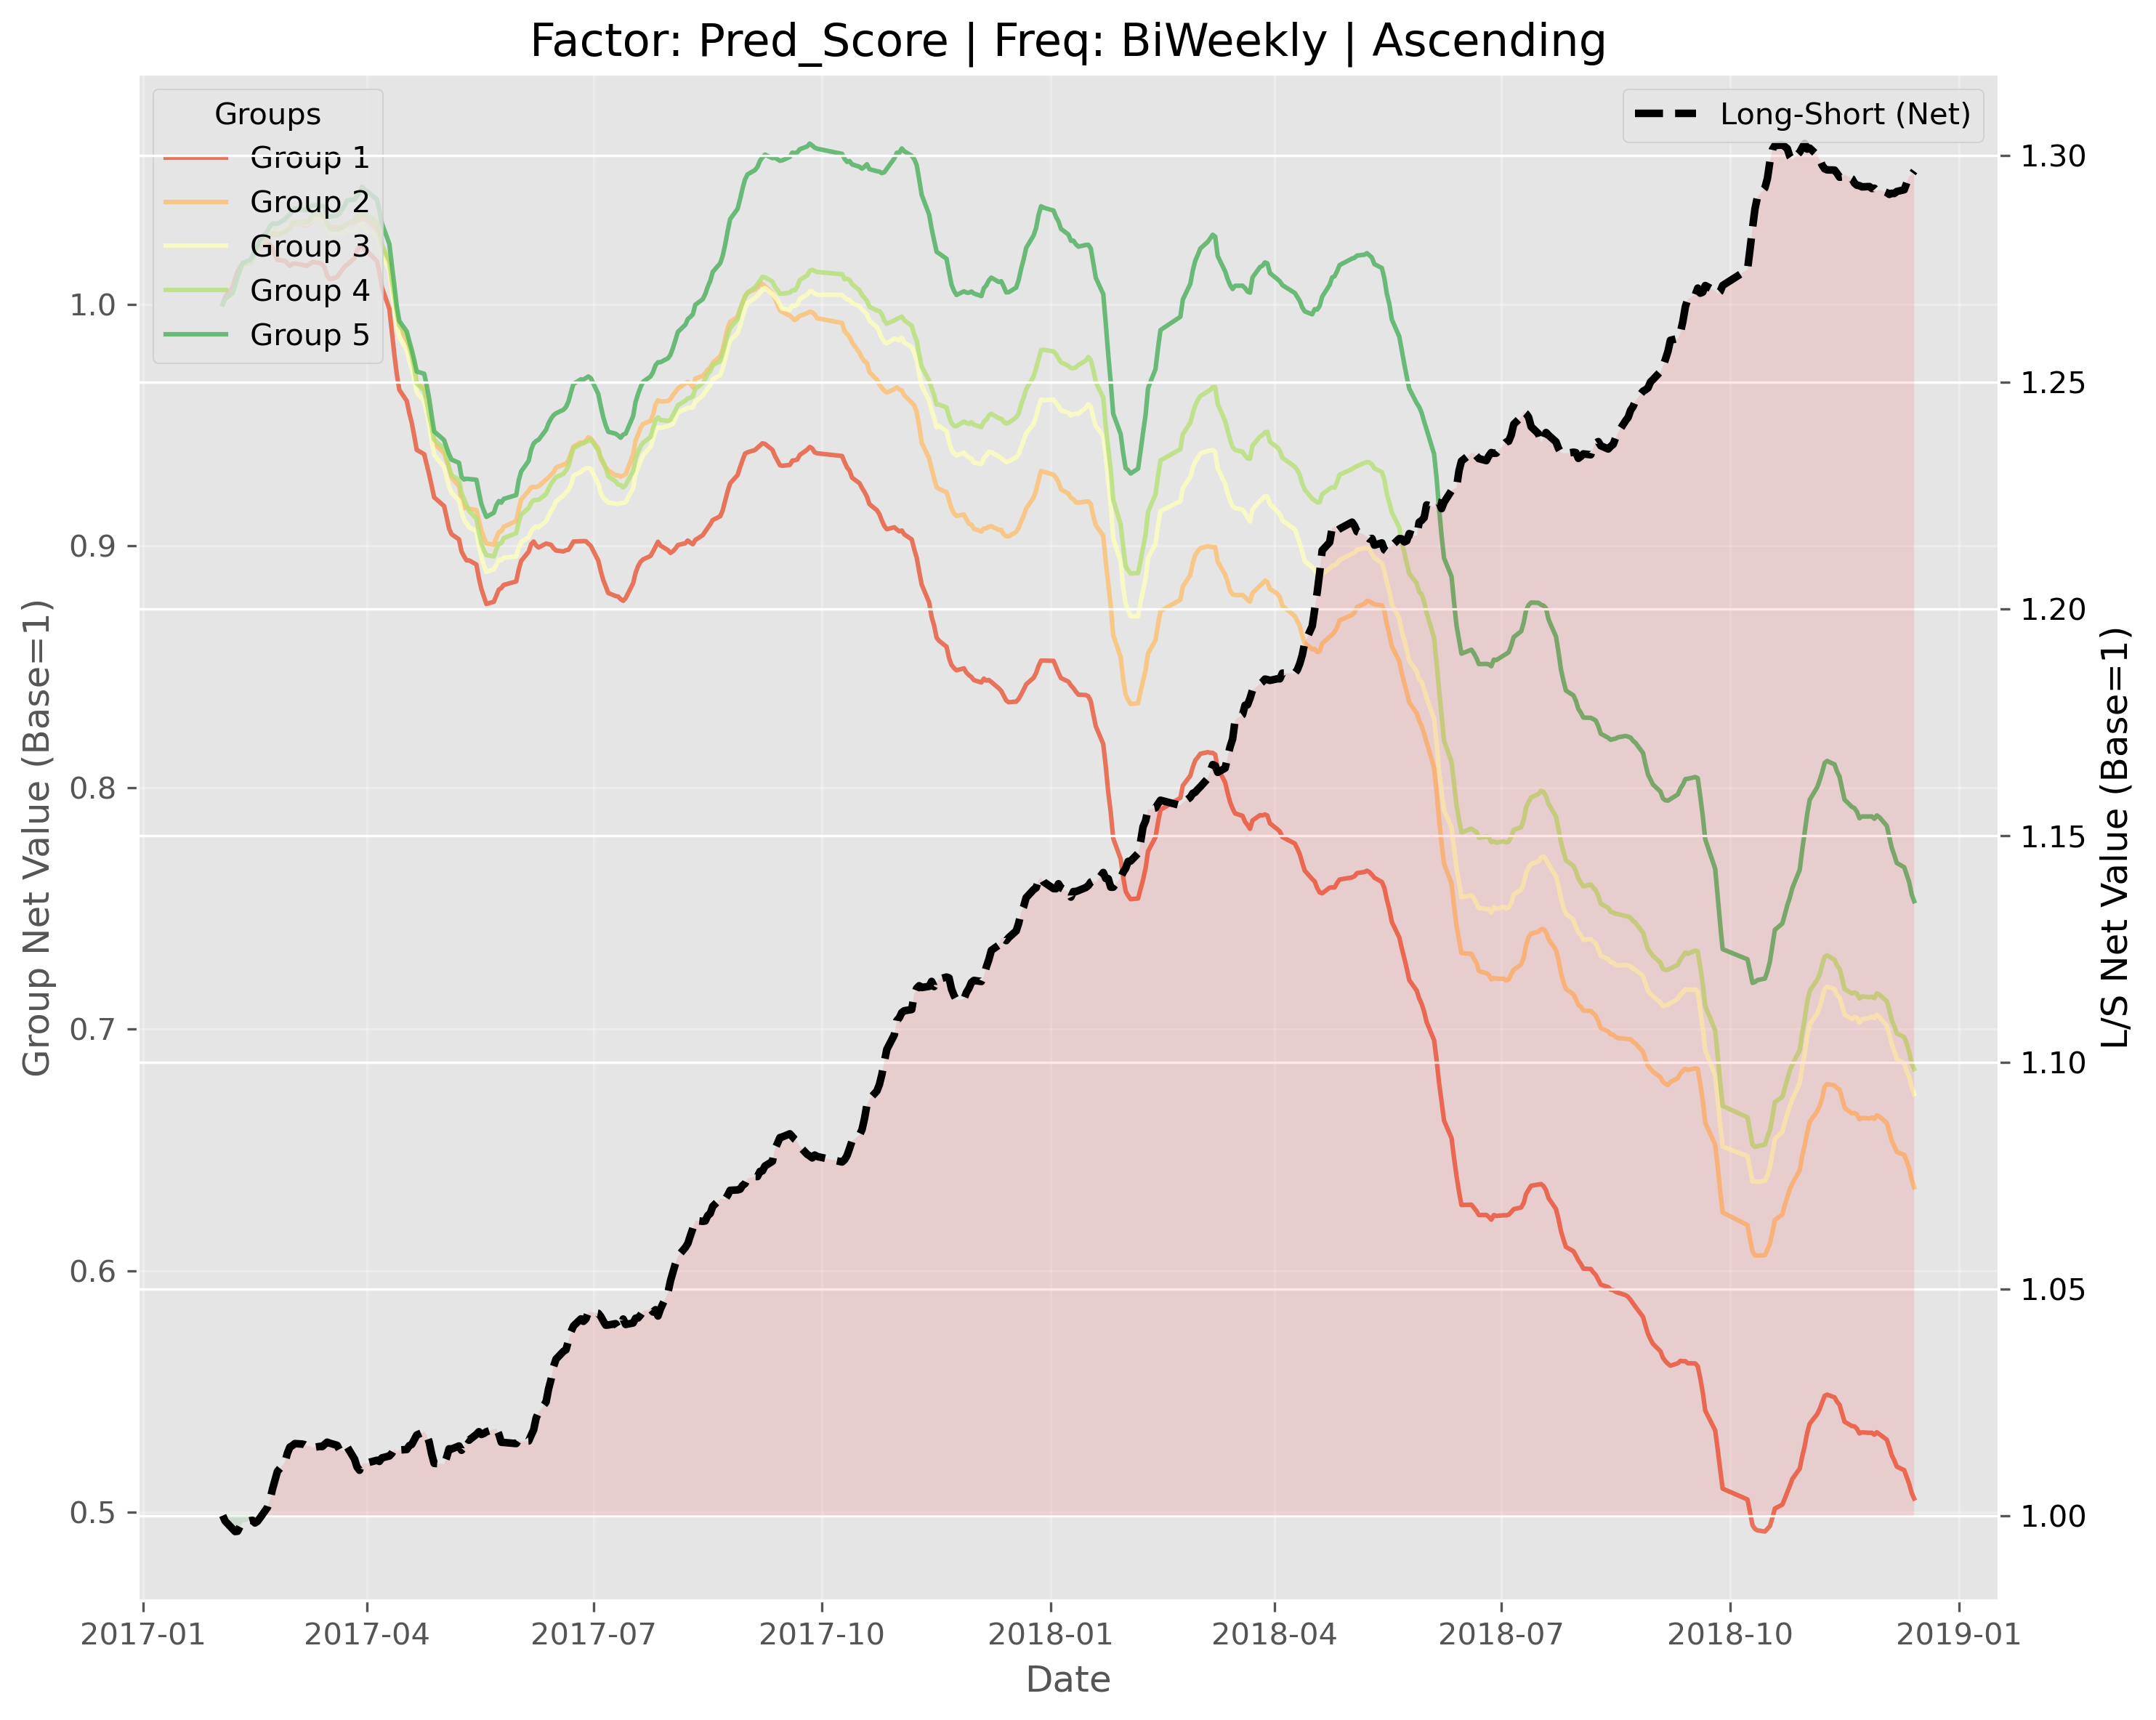
\includegraphics[width=0.6\linewidth]{Factor_Pred_Score_-_Freq_BiWeekly_-_Ascending.png}
\end{figure}

\section{因子思考与改进}

通过对上述因子在不同频率下的实证表现进行复盘，我们发现部分因子的表现呈现出显著的期限结构差异，同时部分经典因子（如Smart Money）的Alpha衰减迹象也值得深思。以下是对核心问题的深度思考与改进方向：

\subsection{对振幅因子（HF\_Amplitude）期限结构倒挂的反思}
实证数据显示，振幅因子在周频（Weekly）策略中失效（年化收益 -2.9\%），但在月频（Monthly）策略中却录得正向收益（7.2\%）。这种“短期反转、长期动量”的矛盾现象揭示了市场微观结构中的分歧机制：
\begin{itemize}
    \item \textbf{短期视角}：在极短周期内，巨大的日内振幅通常代表多空分歧剧烈（Divergence），往往伴随着情绪的宣泄与过热。根据反转效应，此类股票在随后一周面临较大的回调压力。
    \item \textbf{长期视角}：若将观察窗口拉长至一个月，持续的高振幅可能被定价为“高风险特征”。根据资产定价理论，高波动率股票应包含风险溢价（Risk Premium）。
\end{itemize}
\textbf{改进方案：} 为了剥离噪音，建议引入“单位换手带来的振幅”（即Amihud非流动性指标的高频版）。如果一只股票振幅虽大但换手率极低，说明其价格极易被操纵或流动性枯竭，应予以剔除。此外，可尝试将振幅拆解为“上行半方差”与“下行半方差”，以区分良性波动与恶性波动。

\subsection{对偏度因子（HF\_Skewness）强预测性的行为学解释}
日内偏度因子在本研究中表现最为优异（RankIC -0.070）。从行为金融学角度分析，这强有力地验证了A股市场的“博彩效应”（Lottery Preference）。个人投资者倾向于追逐具有正偏度特征（即有小概率暴涨）的“彩票型”股票，导致此类资产在短期内被严重高估，随后必然面临估值回归。
\textbf{改进方案：} 当前计算使用的是总偏度。为了更精准地捕捉Alpha，建议剔除市场因子的影响，计算“特质性偏度”（Idiosyncratic Skewness）。即先用Fama-French三因子模型对分钟收益率进行回归，再对残差序列计算偏度，从而剥离系统性风险带来的不对称性。

\subsection{Smart Money因子的Alpha衰减与优化}
经典的Smart Money因子（S因子）在本回测中虽然有效（年化6.2\%），但相比其他因子表现平庸。这可能源于该因子已被市场广泛使用，导致Alpha衰减。此外，原始算法仅通过成交量占比（前20\%）来定义“聪明钱”，忽略了挂单方向的主动性。
\textbf{改进方案：} 引入Level-2逐笔数据，将“大单主动买入”与“大单被动成交”进行区分。只有主动向上吃单的大额交易才代表强烈的做多意愿。同时，引入时间加权机制，给予尾盘最后30分钟的聪明钱流向更高的权重，因为机构投资者往往在收盘前进行仓位调整。

\section{结论}

本文基于2016年至2018年的高频分钟行情数据，系统性地构建并检验了包含微观资金流向、量价相关性及分布特征在内的多因子体系。研究结论如下：

\begin{enumerate}
    \item \textbf{高频微观结构对低频收益具有显著预测力}：
    实证结果表明，即使在剔除行业、市值、动量及波动率等风格因素后，基于分钟线提取的\texttt{HF\_Skewness}（日内偏度）和\texttt{HF\_CDPDP}（一致性价差）因子依然具备极强的选股能力（月频RankIC均超过5\%）。这证明了A股市场存在显著的非有效性定价，且这种定价偏差主要源于散户的非理性交易行为（如过度追涨、博彩偏好）。

    \item \textbf{因子的正交性与互补性}：
    相关性分析显示，不同类别的高频因子之间相关系数普遍低于0.35。Smart Money捕捉主力意图，CPV捕捉量价情绪，Skewness捕捉博彩偏好，三者在逻辑上互不冲突。这种低相关性为多因子组合提供了天然的优势。

    \item \textbf{非线性模型的组合优势}：
    相比于传统的线性加权，本文采用的XGBoost模型在组合表现上实现了质的飞跃。在双周频换仓下，策略实现了14.8\%的年化超额收益，并将最大回撤控制在2.0\%的极低水平。这说明机器学习模型成功捕捉了因子间的非线性交互效应（例如：在量价背离极度严重时，聪明钱因子的权重可能被动态调整），从而在提升收益的同时显著增强了策略的稳健性。
\end{enumerate}

综上所述，利用高频数据挖掘Alpha并结合机器学习算法进行非线性合成，是构建稳健量化选股策略的有效路径。未来的研究可进一步聚焦于Tick级数据的深度挖掘以及图神经网络（GNN）在股权关联网络中的应用。

\newpage
\section{代码输出}

\begin{lstlisting}
python code2.py
============================================================
Running Pipeline for: CSI500 (Updated for Full Report Replication)
============================================================
>>> [Loader] 加载股票池: ./data/指数权重/index_wt_000905.parquet ...
>>> [Loader] 加载日行情 ...
[Loader] Reading CSVs:   0%|                                                  | 0/10 [00:00<?, ?it/s]Warning: File ./data/日行情/日行情数据字典.csv format mismatch, skipping.
[Loader] Reading CSVs: 100%|█████████████████████████████████████████| 10/10 [00:02<00:00,  3.44it/s]
>>> [Factor] 开始计算高频与滚动因子 (Raw Value Version)...
[Factor] Processing Days: 100%|███████████████████| 731/731 [01:14<00:00,  9.87it/s, date=2018-12-28]
>>> [Factor] 计算完成 (Raw Values)，正在合并...
>>> [Loader] 构造 Labels (Strict Limit Check: Train)...
>>> [Data] Merging Factors and Labels...
>>> [Loader] 加载行业与市值 ...
>>> [Process] 执行特征工程 (Strict Neutralization Mode)...
    [1/4] 计算风格控制变量 (Reversal, Volatility, Turnover)...
    [Info] Constructing 'FloatShares' from 'NonRestrictedShares'...
Debug Columns: ['TradingDay', 'SecuCode', 'HF_SmartMoney', 'HF_Raw_CPV_Mean', 'HF_CDPDP', 'HF_Skewness', 'HF_Tail_Reversal', 'HF_Amplitude', 'ClosePrice', 'OpenPrice', 'Volume', 'Amount', 'NonRestrictedShares', 'AFloats', 'PTFlag', 'Next_Open', 'Next_PTFlag', 'Next_Next_Open', 'SettlementDate', 'Limit_Threshold', 'Next_Open_Chg', 'Ret_Hold', 'InfoPublDate', 'tag', 'Industry', 'LnCap', 'Ctrl_Ret20', 'Ctrl_Vol20', 'FloatShares']
    [Info] Turnover calculated using NonRestrictedShares/AFloats.
    [2/4] 计算 Label 行业相对收益...
    [3/4] 分批特征处理 (Batch -> Orthogonalization -> Disk)...
Processing Batches: 100%|████████████████████████████████████████████| 36/36 [00:06<00:00,  5.63it/s]
    [4/4] 合并最终数据集...
>>> [Model] 开始滚动训练 (Detailed Metrics: IC, RankIC, L/S Ret, Sharpe, Turnover)...
Pred: 2017-02 | IC: 0.0211 | RankIC: 0.0359 | L/S AnnRet: 26.02% | Sharpe: 3.86 | Turnover: 31.89%   
Pred: 2017-03 | IC: 0.0255 | RankIC: 0.0295 | L/S AnnRet: 21.59% | Sharpe: 2.55 | Turnover: 34.17%   
Pred: 2017-04 | IC: 0.0266 | RankIC: 0.0314 | L/S AnnRet: 63.76% | Sharpe: 5.53 | Turnover: 35.78%   
Pred: 2017-05 | IC: 0.0148 | RankIC: 0.0088 | L/S AnnRet: -0.43% | Sharpe: -0.04 | Turnover: 32.70%  
Pred: 2017-06 | IC: 0.0350 | RankIC: 0.0616 | L/S AnnRet: 59.21% | Sharpe: 7.33 | Turnover: 29.91%   
Pred: 2017-07 | IC: 0.0134 | RankIC: 0.0395 | L/S AnnRet: 10.66% | Sharpe: 0.76 | Turnover: 30.95%   
Pred: 2017-08 | IC: 0.0328 | RankIC: 0.0463 | L/S AnnRet: 87.53% | Sharpe: 11.98 | Turnover: 32.00%  
Pred: 2017-09 | IC: -0.0014 | RankIC: 0.0341 | L/S AnnRet: 13.74% | Sharpe: 2.32 | Turnover: 30.29%  
Pred: 2017-10 | IC: 0.0205 | RankIC: 0.0312 | L/S AnnRet: 28.47% | Sharpe: 3.70 | Turnover: 35.06%   
Pred: 2017-11 | IC: 0.0171 | RankIC: 0.0222 | L/S AnnRet: 36.16% | Sharpe: 3.25 | Turnover: 31.64%   
Pred: 2017-12 | IC: 0.0648 | RankIC: 0.0563 | L/S AnnRet: 96.57% | Sharpe: 9.71 | Turnover: 33.14%   
Pred: 2018-01 | IC: 0.0082 | RankIC: 0.0120 | L/S AnnRet: -20.36% | Sharpe: -2.27 | Turnover: 32.00% 
Pred: 2018-02 | IC: 0.0316 | RankIC: 0.0332 | L/S AnnRet: 81.86% | Sharpe: 7.50 | Turnover: 33.07%   
Pred: 2018-03 | IC: 0.0054 | RankIC: 0.0177 | L/S AnnRet: 50.24% | Sharpe: 3.92 | Turnover: 34.64%   
Pred: 2018-04 | IC: 0.0354 | RankIC: 0.0384 | L/S AnnRet: 64.50% | Sharpe: 7.35 | Turnover: 34.00%   
Pred: 2018-05 | IC: 0.0154 | RankIC: 0.0268 | L/S AnnRet: 33.24% | Sharpe: 3.69 | Turnover: 31.91%   
Pred: 2018-06 | IC: 0.0315 | RankIC: 0.0442 | L/S AnnRet: 116.80% | Sharpe: 15.32 | Turnover: 33.10% 
Pred: 2018-07 | IC: 0.0026 | RankIC: -0.0016 | L/S AnnRet: 9.59% | Sharpe: 0.99 | Turnover: 36.09%   
Pred: 2018-08 | IC: 0.0316 | RankIC: 0.0241 | L/S AnnRet: 51.13% | Sharpe: 4.40 | Turnover: 37.39%   
Pred: 2018-09 | IC: 0.0242 | RankIC: 0.0269 | L/S AnnRet: 46.21% | Sharpe: 5.92 | Turnover: 37.68%   
Pred: 2018-10 | IC: 0.0343 | RankIC: 0.0382 | L/S AnnRet: 86.54% | Sharpe: 6.35 | Turnover: 35.44%   
Pred: 2018-11 | IC: 0.0122 | RankIC: 0.0271 | L/S AnnRet: 23.55% | Sharpe: 2.62 | Turnover: 37.73%   
Pred: 2018-12 | IC: 0.0375 | RankIC: 0.0429 | L/S AnnRet: 55.67% | Sharpe: 8.60 | Turnover: 36.44%   
[Model] Walk-Forward: 100%|██████████████████████████████████████████| 24/24 [00:04<00:00,  5.33it/s]
--- Plotting Correlation Matrix (spearman) ---
>>> Plot saved to: ./plots/Factor_Correlation_Matrix_(Pre-Model)_spearman.png

============================================================
Starting Factor Analysis (Corrected Direction & Extended Metrics)
============================================================
>>> [Analyzer] Calculating Forward Returns for Multi-Period Testing...

>>> Analyzing Factor: HF_SmartMoney [Descending]
>>> Plot saved to: ./plots/Factor_HF_SmartMoney_-_Freq_Weekly_-_Descending.png
  [Weekly  ] IC:-0.041 | RankIC:-0.057 | Ret:6.4% | R/V:1.18 | MaxDD:-4.0% | Turn:0.53
>>> Plot saved to: ./plots/Factor_HF_SmartMoney_-_Freq_BiWeekly_-_Descending.png
  [BiWeekly] IC:-0.038 | RankIC:-0.058 | Ret:5.8% | R/V:0.97 | MaxDD:-7.4% | Turn:0.76
>>> Plot saved to: ./plots/Factor_HF_SmartMoney_-_Freq_Monthly_-_Descending.png
  [Monthly ] IC:-0.037 | RankIC:-0.052 | Ret:6.2% | R/V:1.11 | MaxDD:-7.5% | Turn:0.77

>>> Analyzing Factor: HF_Raw_CPV_Mean [Descending]
>>> Plot saved to: ./plots/Factor_HF_Raw_CPV_Mean_-_Freq_Weekly_-_Descending.png
  [Weekly  ] IC:-0.039 | RankIC:-0.051 | Ret:7.7% | R/V:1.30 | MaxDD:-3.9% | Turn:0.38
>>> Plot saved to: ./plots/Factor_HF_Raw_CPV_Mean_-_Freq_BiWeekly_-_Descending.png
  [BiWeekly] IC:-0.044 | RankIC:-0.056 | Ret:11.4% | R/V:1.91 | MaxDD:-3.3% | Turn:0.54
>>> Plot saved to: ./plots/Factor_HF_Raw_CPV_Mean_-_Freq_Monthly_-_Descending.png
  [Monthly ] IC:-0.047 | RankIC:-0.059 | Ret:11.8% | R/V:2.14 | MaxDD:-3.7% | Turn:0.75

>>> Analyzing Factor: HF_CDPDP [Descending]
>>> Plot saved to: ./plots/Factor_HF_CDPDP_-_Freq_Weekly_-_Descending.png
  [Weekly  ] IC:-0.029 | RankIC:-0.044 | Ret:4.1% | R/V:0.58 | MaxDD:-10.9% | Turn:0.26
>>> Plot saved to: ./plots/Factor_HF_CDPDP_-_Freq_BiWeekly_-_Descending.png
  [BiWeekly] IC:-0.039 | RankIC:-0.057 | Ret:12.3% | R/V:1.70 | MaxDD:-7.4% | Turn:0.38
>>> Plot saved to: ./plots/Factor_HF_CDPDP_-_Freq_Monthly_-_Descending.png
  [Monthly ] IC:-0.044 | RankIC:-0.064 | Ret:12.2% | R/V:1.99 | MaxDD:-3.8% | Turn:0.55

>>> Analyzing Factor: HF_Skewness [Descending]
>>> Plot saved to: ./plots/Factor_HF_Skewness_-_Freq_Weekly_-_Descending.png
  [Weekly  ] IC:-0.037 | RankIC:-0.053 | Ret:6.8% | R/V:1.28 | MaxDD:-4.3% | Turn:0.35
>>> Plot saved to: ./plots/Factor_HF_Skewness_-_Freq_BiWeekly_-_Descending.png
  [BiWeekly] IC:-0.045 | RankIC:-0.059 | Ret:11.8% | R/V:2.25 | MaxDD:-2.6% | Turn:0.50
>>> Plot saved to: ./plots/Factor_HF_Skewness_-_Freq_Monthly_-_Descending.png
  [Monthly ] IC:-0.054 | RankIC:-0.070 | Ret:12.6% | R/V:2.60 | MaxDD:-3.7% | Turn:0.72

>>> Analyzing Factor: HF_Tail_Reversal [Descending]
>>> Plot saved to: ./plots/Factor_HF_Tail_Reversal_-_Freq_Weekly_-_Descending.png
  [Weekly  ] IC:-0.034 | RankIC:-0.033 | Ret:4.9% | R/V:0.81 | MaxDD:-8.1% | Turn:0.35
>>> Plot saved to: ./plots/Factor_HF_Tail_Reversal_-_Freq_BiWeekly_-_Descending.png
  [BiWeekly] IC:-0.035 | RankIC:-0.030 | Ret:5.3% | R/V:0.89 | MaxDD:-8.6% | Turn:0.50
>>> Plot saved to: ./plots/Factor_HF_Tail_Reversal_-_Freq_Monthly_-_Descending.png
  [Monthly ] IC:-0.033 | RankIC:-0.028 | Ret:5.1% | R/V:0.89 | MaxDD:-7.2% | Turn:0.71

>>> Analyzing Factor: HF_Amplitude [Descending]
>>> Plot saved to: ./plots/Factor_HF_Amplitude_-_Freq_Weekly_-_Descending.png
  [Weekly  ] IC:-0.021 | RankIC:-0.045 | Ret:-2.9% | R/V:-0.30 | MaxDD:-23.3% | Turn:0.18
>>> Plot saved to: ./plots/Factor_HF_Amplitude_-_Freq_BiWeekly_-_Descending.png
  [BiWeekly] IC:-0.030 | RankIC:-0.054 | Ret:4.0% | R/V:0.42 | MaxDD:-13.9% | Turn:0.29
>>> Plot saved to: ./plots/Factor_HF_Amplitude_-_Freq_Monthly_-_Descending.png
  [Monthly ] IC:-0.038 | RankIC:-0.066 | Ret:7.2% | R/V:0.86 | MaxDD:-10.2% | Turn:0.44

>>> Analyzing Factor: Pred_Score [Ascending]
>>> Plot saved to: ./plots/Factor_Pred_Score_-_Freq_Weekly_-_Ascending.png
  [Weekly  ] IC:0.046 | RankIC:0.050 | Ret:10.8% | R/V:1.78 | MaxDD:-3.6% | Turn:0.47
>>> Plot saved to: ./plots/Factor_Pred_Score_-_Freq_BiWeekly_-_Ascending.png
  [BiWeekly] IC:0.045 | RankIC:0.045 | Ret:14.8% | R/V:2.61 | MaxDD:-2.0% | Turn:0.58
>>> Plot saved to: ./plots/Factor_Pred_Score_-_Freq_Monthly_-_Ascending.png
  [Monthly ] IC:0.029 | RankIC:0.045 | Ret:8.5% | R/V:1.65 | MaxDD:-4.4% | Turn:0.71
--- Plotting Correlation Matrix (spearman) ---
>>> Plot saved to: ./plots/Factor_Correlation_Matrix_spearman.png
\end{lstlisting}

% 参考文献
\clearpage
\reference
\end{document}


